\documentclass[12pt,a4paper]{article}

% Packages
\usepackage[utf8]{inputenc}
\usepackage[T1]{fontenc}
\usepackage{lmodern}
\usepackage[margin=1in]{geometry}
\usepackage{graphicx}
\usepackage{hyperref}
\usepackage{booktabs}
\usepackage{enumitem}
\usepackage{xcolor}
\usepackage{titlesec}
\usepackage{fancyhdr}
\usepackage{float}
\usepackage{parskip}

% Colors
\definecolor{udacityblue}{HTML}{02B3E4}
\definecolor{sectionblue}{HTML}{1A73E8}

% Header/Footer
\pagestyle{fancy}
\fancyhf{}
\fancyhead[L]{\small AI Vectra Bank -- Multi-Agent RAG System}
\fancyhead[R]{\small Udacity -- Microsoft Azure AI Foundry}
\fancyfoot[C]{\thepage}
\renewcommand{\headrulewidth}{0.4pt}

% Section formatting
\titleformat{\section}{\Large\bfseries\color{sectionblue}}{}{0em}{}
\titleformat{\subsection}{\large\bfseries}{}{0em}{}
\titleformat{\subsubsection}{\normalsize\bfseries}{}{0em}{}

% Graphics path
\graphicspath{{screenshots/}}

% Hyperref setup
\hypersetup{
    colorlinks=true,
    linkcolor=sectionblue,
    urlcolor=udacityblue,
    pdftitle={AI Vectra Bank -- Banking Multi-Agent RAG System},
    pdfauthor={Rodolfo Lerma Contreras}
}

\begin{document}

% ============================================================================
% TITLE PAGE
% ============================================================================
\begin{titlepage}
\centering
\vspace*{2cm}

{\Huge\bfseries AI Vectra Bank\par}
\vspace{0.5cm}
{\LARGE Banking Multi-Agent RAG System\par}
\vspace{1.5cm}
{\Large\color{sectionblue} Microsoft Azure AI Foundry Nanodegree\par}
{\large Udacity -- Project 4\par}
\vspace{2cm}
{\large Rodolfo Lerma Contreras\par}
\vspace{0.5cm}
{\large February 2026\par}
\vspace{2cm}

\noindent\rule{0.8\textwidth}{0.4pt}
\vspace{0.5cm}

{\normalsize
Repository: \url{https://github.com/rodolfolermacontreras/AI-Vectra-Bank-AI-Agentic-RAG-for-Banking}\par
}

\vfill
\end{titlepage}

% ============================================================================
% TABLE OF CONTENTS
% ============================================================================
\tableofcontents
\newpage

% ============================================================================
% 1. PROJECT OVERVIEW
% ============================================================================
\section{Project Overview}

This project implements a multi-agent banking intelligence system that
orchestrates six specialised AI agents using Microsoft Semantic Kernel.
The system processes complex banking queries through a sequential pipeline
where each agent contributes domain-specific analysis, ultimately producing
a comprehensive financial report.

The six agents are:
\begin{enumerate}
    \item \textbf{Data Gatherer} -- retrieves customer data from Azure SQL Database
    \item \textbf{Fraud Analyst} -- analyses transaction patterns for suspicious activity
    \item \textbf{Loan Analyst} -- evaluates loan eligibility and credit risk
    \item \textbf{Support Specialist} -- provides customer support recommendations
    \item \textbf{Risk Analyst} -- performs comprehensive risk assessment using RAG
    \item \textbf{Synthesis Coordinator} -- integrates all findings into a final report
\end{enumerate}

% ============================================================================
% 2. DESIGN DECISIONS
% ============================================================================
\section{Design Decisions}

\subsection{Sequential Orchestration Pattern}

I chose sequential (pipeline) orchestration over parallel execution because
each agent's output enriches the context for the next agent. For example,
the Fraud Analyst needs transaction data from the Data Gatherer, and the
Risk Analyst needs fraud and loan findings to produce a meaningful risk
assessment. This sequential dependency makes a pipeline the natural fit.

The trade-off is latency -- a full run takes approximately 60 seconds because
each agent waits for its predecessor. However, the quality improvement from
accumulated context outweighs the performance cost for a banking use case
where thoroughness matters more than speed.

\subsection{Azure OpenAI Embeddings for RAG}

The project required using Azure-hosted embeddings rather than ChromaDB's
default embedding function. I implemented a custom
\texttt{AzureOpenAIEmbeddingFunction} class that integrates with the Azure OpenAI
\texttt{text-embedding-ada-002} model (1536 dimensions). This class implements
ChromaDB's \texttt{EmbeddingFunction} protocol, allowing seamless drop-in replacement.

Key design choice: I used the REST API directly (via the \texttt{openai} Python SDK)
rather than the Azure AI Inference SDK, because \texttt{text-embedding-ada-002}
requires the \texttt{2024-06-01} API version which maps cleanly to the OpenAI
client's \texttt{AzureOpenAI} class.

\subsection{Azure SQL Database for Customer Data}

Rather than relying solely on sample/mock data, I provisioned a live Azure
SQL Database (\texttt{vectra-bank-db}) with 12 transaction records across 3 customer
profiles. The \texttt{DataConnector} class implements graceful fallback -- if the
Azure SQL connection is unavailable, it falls back to sample data, ensuring
the system works both online and offline.

\subsection{Pydantic Models for Structured Output}

All agent outputs are captured in Pydantic models (\texttt{CustomerProfile},
\texttt{EnhancedBankingReport}) with field validation. This ensures type safety,
automatic serialisation to JSON for report storage, and clear contracts
between agents. Risk scores are clamped to 0--100, credit scores to 300--850,
and enums enforce valid status values.

\subsection{Six ChromaDB Collections}

I organised the vector store into six topic-specific collections
(fraud\_detection, loan\_policies, customer\_support, risk\_assessment,
transaction\_monitoring, compliance) rather than a single collection. This
improves retrieval relevance because semantic search is scoped to the
appropriate policy domain for each agent.

% ============================================================================
% 3. CHALLENGES AND SOLUTIONS
% ============================================================================
\section{Challenges and Solutions}

\subsection{Python Version Compatibility}

\textbf{Challenge}: Initially attempted Python 3.14, but \texttt{pydantic-core}
failed to build from source (no pre-compiled wheel available).

\textbf{Solution}: Downgraded to Python 3.12, which has pre-built wheels for all
dependencies including \texttt{chromadb}, \texttt{semantic-kernel}, and \texttt{pydantic}.

\subsection{Windows Console Encoding (cp1252)}

\textbf{Challenge}: The seed code files contained Unicode emoji characters that
crash on Windows PowerShell terminals using cp1252 encoding. This caused 16 of
23 tests to fail silently with \texttt{UnicodeEncodeError}.

\textbf{Solution}: Replaced all emoji characters with ASCII equivalents
(\texttt{[OK]}, \texttt{[FAIL]}, \texttt{[ERROR]}). This is documented in
\texttt{DEVELOPMENT\_RULES.md} as a project-wide standard.

\subsection{Azure Region Availability}

\textbf{Challenge}: Azure SQL Server creation failed in \texttt{eastus} with a
capacity error -- the region was blocked for the Udacity subscription.

\textbf{Solution}: Deployed to \texttt{westus} instead. This required no code changes
since the ODBC connection string abstracts the server location.

\subsection{Azure Embedding API Version}

\textbf{Challenge}: The \texttt{text-embedding-ada-002} model requires API version
\texttt{2024-06-01}. Using newer versions returned 404 errors.

\textbf{Solution}: Hard-coded \texttt{api\_version="2024-06-01"} in the
\texttt{AzureOpenAIEmbeddingFunction} class.

\subsection{ChromaDB Stale State}

\textbf{Challenge}: After switching Azure credentials, the local ChromaDB contained
vectors generated with old embedding keys, causing dimension mismatches.

\textbf{Solution}: Deleted the stale \texttt{chroma\_db\_banking/} directory to force a
clean rebuild on next run.

% ============================================================================
% 4. WHAT I LEARNED
% ============================================================================
\section{What I Learned}

\subsection{Multi-Agent Orchestration}
Building a six-agent system taught me that agent design is as much about
\textbf{prompt engineering} as it is about code. Each agent's system prompt must
clearly define its scope, expected inputs, and output format.

\subsection{RAG Pipeline Design}
Implementing RAG with Azure embeddings and ChromaDB reinforced that
\textbf{chunking strategy} matters enormously. Banking policy documents needed
to be split at logical boundaries rather than fixed character counts.

\subsection{Azure Service Integration}
Working with Azure AI Foundry, Azure SQL, and Azure OpenAI simultaneously
taught me the importance of \textbf{environment configuration management}.
Using \texttt{.env} files with \texttt{python-dotenv} and providing clear
\texttt{env.example} templates makes the project reproducible.

\subsection{Testing Strategy}
The 23-test suite covers models, connectors, embeddings, ChromaDB, RAG, SQL,
and orchestration. Having comprehensive tests caught the emoji encoding issue
immediately and verified that all Azure integrations were live.

% ============================================================================
% 5. EVALUATION RESULTS
% ============================================================================
\section{Evaluation Results}

\subsection{Test Suite (23/23 Pass)}

All 23 automated tests pass with live Azure services:
\begin{itemize}
    \item Model validation tests (5): Pydantic model creation and constraints
    \item Blob storage tests (3): Document upload and retrieval
    \item Embedding tests (2): Azure embedding generation (1536-dim vectors)
    \item ChromaDB tests (3): Collection management and document storage
    \item RAG tests (1): Semantic search with Azure embeddings
    \item SQL tests (3): Live Azure SQL connection, income and transaction queries
    \item Orchestration tests (6): Agent creation, naming, policy extraction
\end{itemize}

\subsection{Evaluation Suite (5/5 Scenarios Pass)}

\begin{table}[H]
\centering
\begin{tabular}{ccccc}
\toprule
\textbf{Scenario} & \textbf{Customer} & \textbf{Risk Score} & \textbf{Assessment} & \textbf{Agents} \\
\midrule
1 & 12345 & 12/100 & Low & 6/6 \\
2 & 67890 & 52/100 & High & 6/6 \\
3 & 11111 & 94/100 & Critical & 6/6 \\
4 & 12345 & 12/100 & Low & 6/6 \\
5 & 67890 & 52/100 & High & 6/6 \\
\bottomrule
\end{tabular}
\caption{Evaluation results across all 5 scenarios}
\end{table}

The risk scores appropriately differentiate between customer profiles:
\begin{itemize}
    \item Customer 12345 (\$75K income, 780 credit) = consistently low risk
    \item Customer 67890 (\$45K income, 620 credit) = consistently high risk
    \item Customer 11111 (\$28K income, 520 credit) = consistently critical risk
\end{itemize}

% ============================================================================
% 6. ARCHITECTURE DECISIONS SUMMARY
% ============================================================================
\section{Architecture Decisions Summary}

\begin{table}[H]
\centering
\begin{tabular}{lll}
\toprule
\textbf{Decision} & \textbf{Choice} & \textbf{Rationale} \\
\midrule
Orchestration & Sequential pipeline & Agent outputs depend on predecessors \\
LLM & gpt-4o (2024-11-20) & Best balance of quality and speed \\
Embeddings & text-embedding-ada-002 & Rubric requirement; 1536-dim \\
Vector DB & ChromaDB (6 collections) & Lightweight, topic-scoped retrieval \\
SQL & Azure SQL Database & Live customer data with fallback \\
Framework & Semantic Kernel & Native Azure integration \\
Models & Pydantic v2 & Type safety, validation, JSON \\
Testing & Built-in test harness & 23 tests covering all integrations \\
\bottomrule
\end{tabular}
\caption{Architecture decisions summary}
\end{table}

% ============================================================================
% 7. SUGGESTIONS FOR IMPROVEMENT
% ============================================================================
\section{Suggestions for Improvement}

\subsection{Parallel Agent Execution with Dependency Awareness}

The current sequential pipeline takes approximately 60 seconds per scenario
because each agent waits for its predecessor to finish. In practice, some
agents are partially independent -- the Fraud Analyst and Loan Analyst both
depend on the Data Gatherer but not on each other. Introducing a
\textbf{dependency-aware parallel scheduler} (e.g., a DAG-based execution engine)
would allow Fraud and Loan analysis to run concurrently once the Data
Gatherer completes. Based on observed timings, this could reduce end-to-end
latency by 30--40\%, bringing it closer to 35--40 seconds per scenario.

\subsection{Conversation Memory for Multi-Turn Interactions}

The system currently treats every query as a one-shot interaction -- there is
no memory of previous conversations. Adding a \textbf{session-based conversation
memory} (e.g., using Semantic Kernel's chat history or an external store like
Redis) would allow agents to reference prior context, avoid redundant data
fetches, and deliver more natural multi-turn dialogues.

% ============================================================================
% 8. CONCLUSION
% ============================================================================
\section{Conclusion}

This project demonstrates a production-quality multi-agent banking system
that integrates Azure AI Foundry (GPT-4o), Azure OpenAI Embeddings
(text-embedding-ada-002), Azure SQL Database, and ChromaDB for RAG-based
policy retrieval. The sequential orchestration pattern ensures each agent
builds on accumulated context, producing thorough and contextually relevant
banking analysis reports.

The system successfully differentiates between low-risk, high-risk, and
critical-risk customer profiles, with risk scores that accurately reflect
each customer's financial situation. All 23 tests pass with live Azure
services, and all 5 evaluation scenarios complete successfully with all 6
agents activated.

% ============================================================================
% SCREENSHOTS -- AZURE RESOURCES
% ============================================================================
\newpage
\section{Appendix A: Azure Resource Screenshots}

\subsection{Azure OpenAI -- Overview}
\begin{figure}[H]
\centering
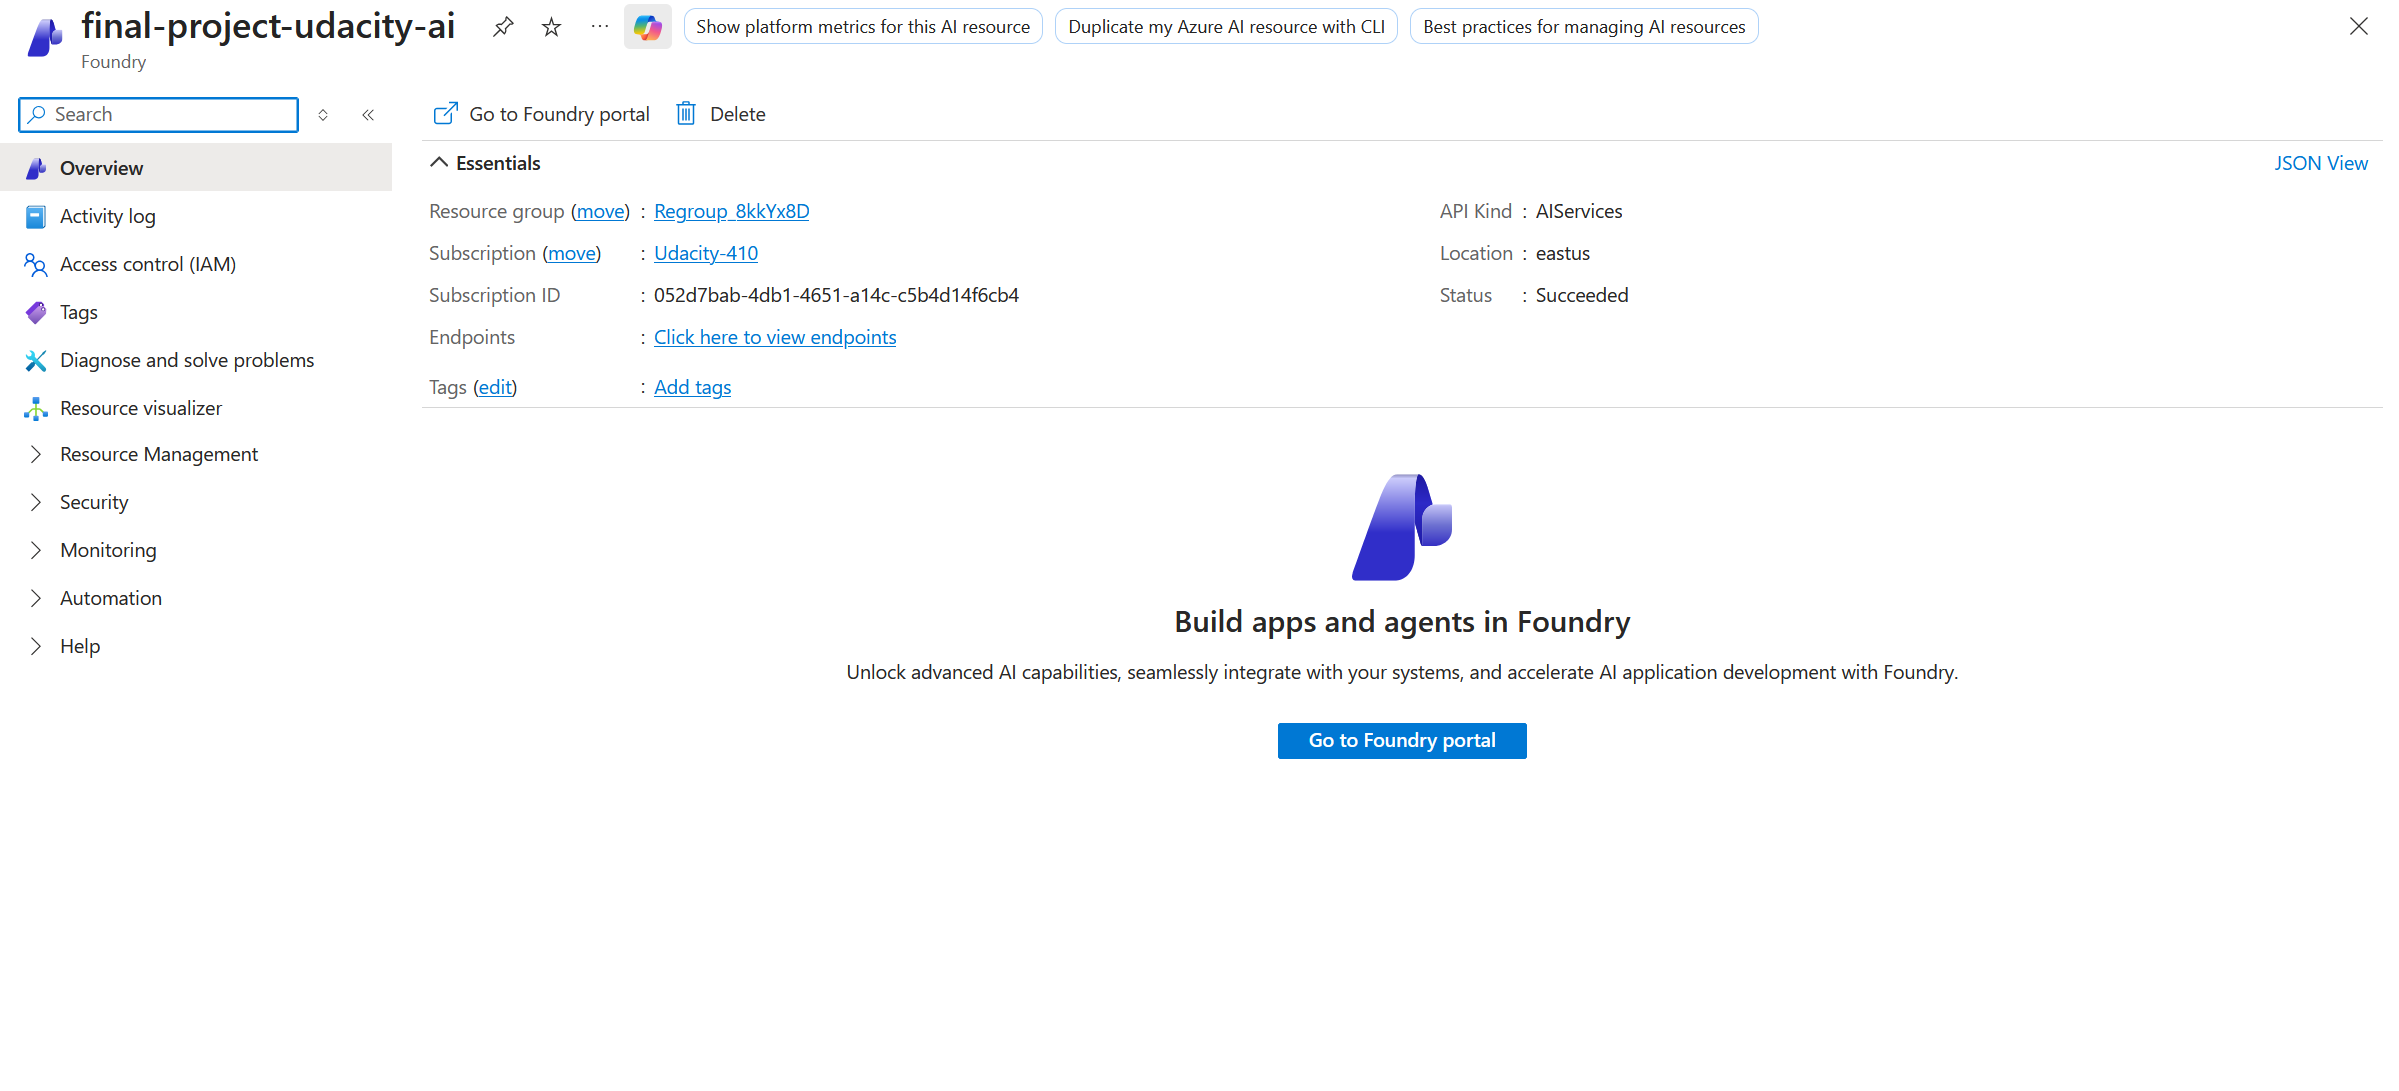
\includegraphics[width=\textwidth]{azure_openai_overview.png}
\caption{Azure OpenAI Service -- Resource Overview}
\end{figure}

\subsection{Azure OpenAI -- Model Deployments}
\begin{figure}[H]
\centering
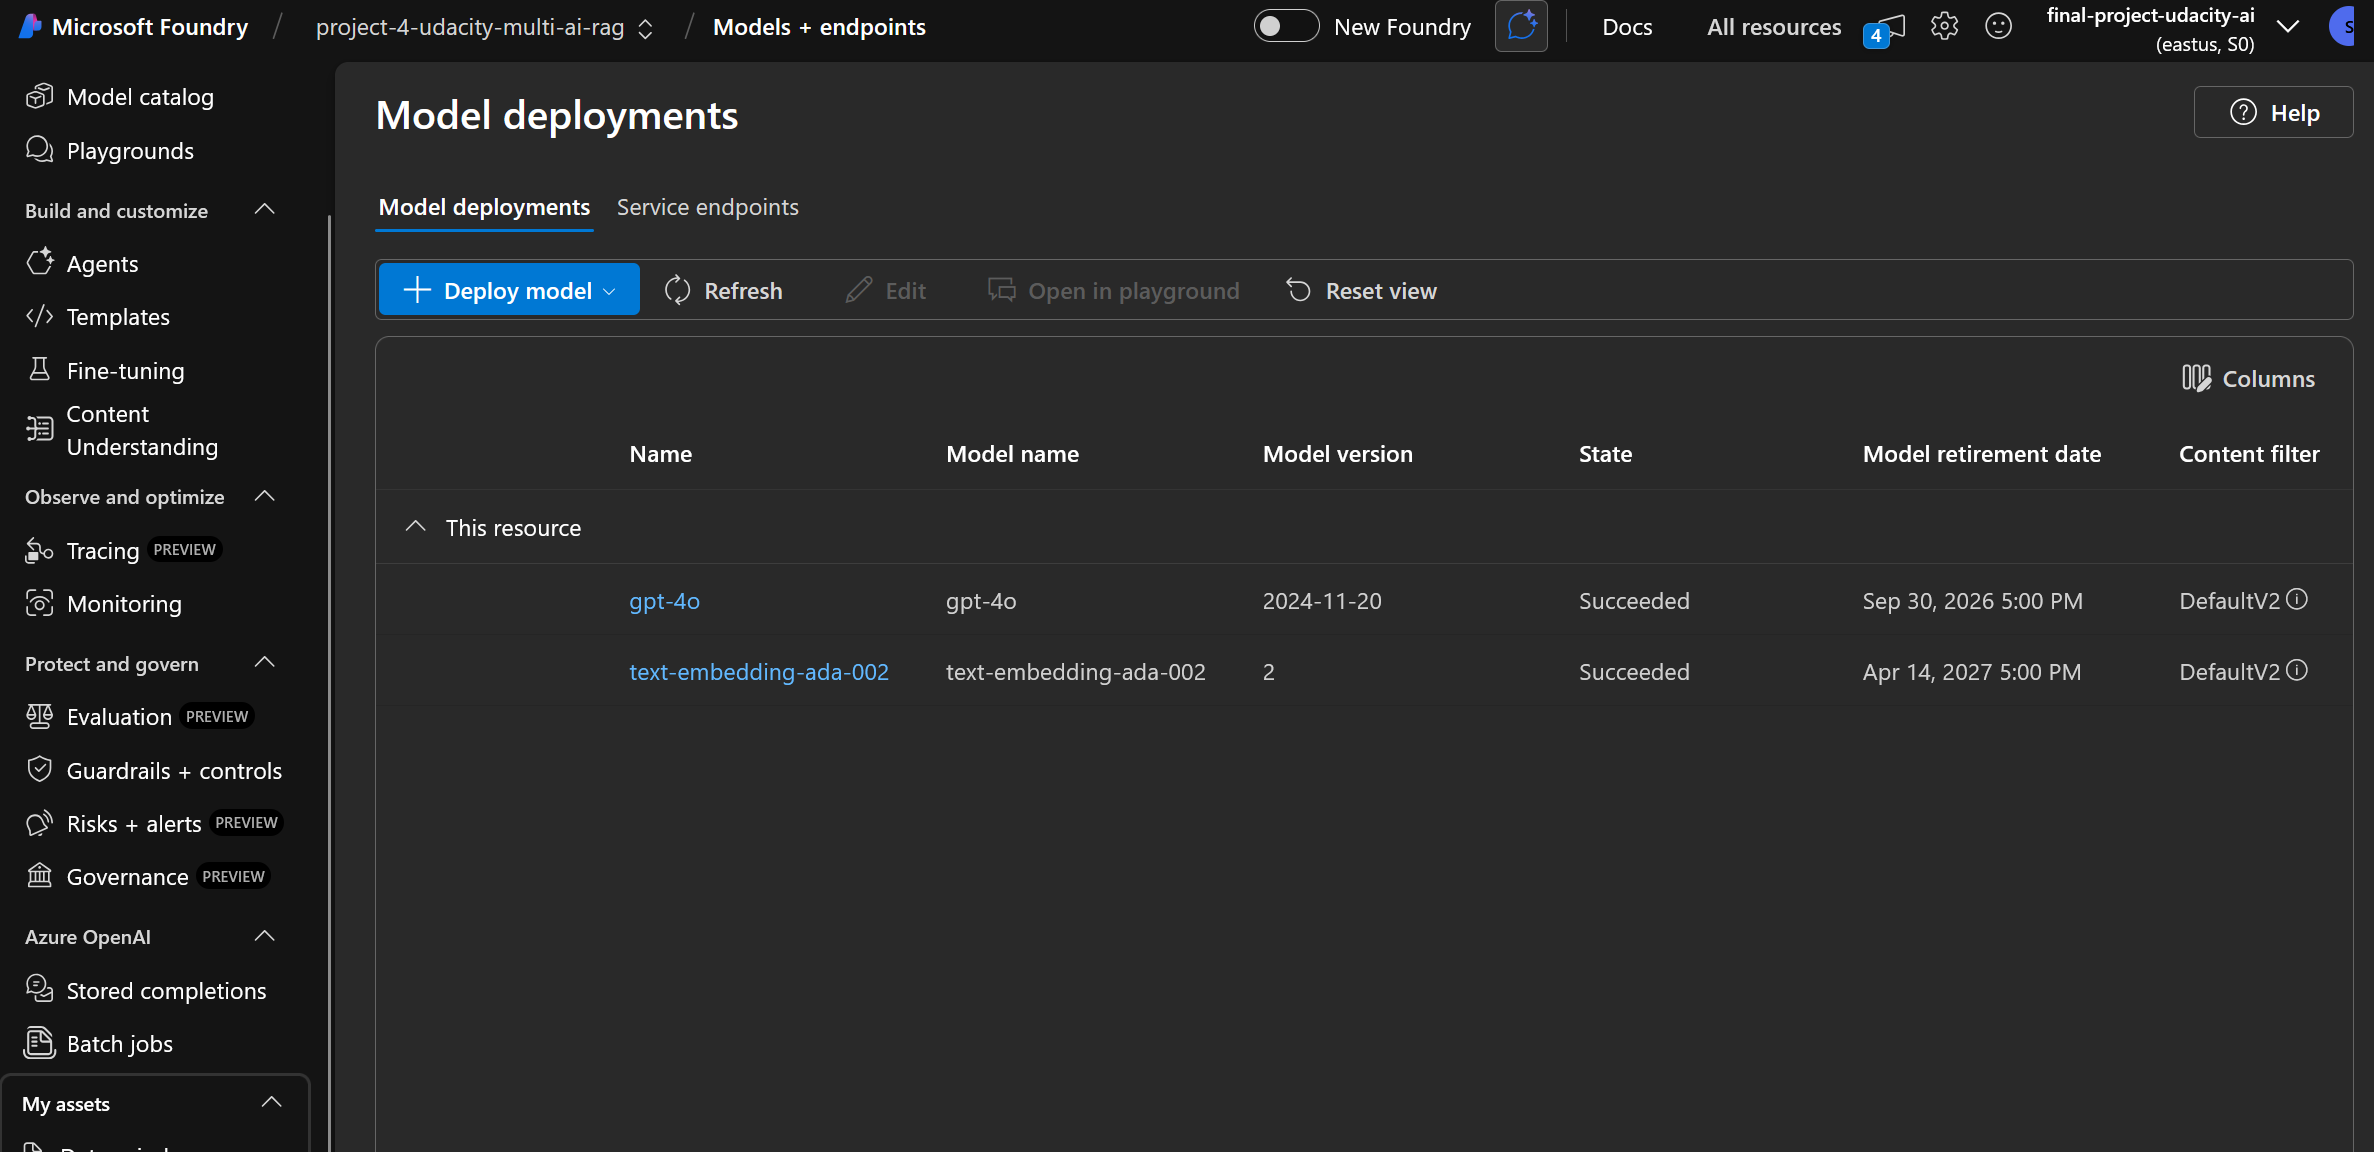
\includegraphics[width=\textwidth]{azure_openai_deployments.png}
\caption{Azure OpenAI -- Model Deployments (gpt-4o + text-embedding-ada-002)}
\end{figure}

\subsection{Azure OpenAI -- Keys and Endpoint}
\begin{figure}[H]
\centering
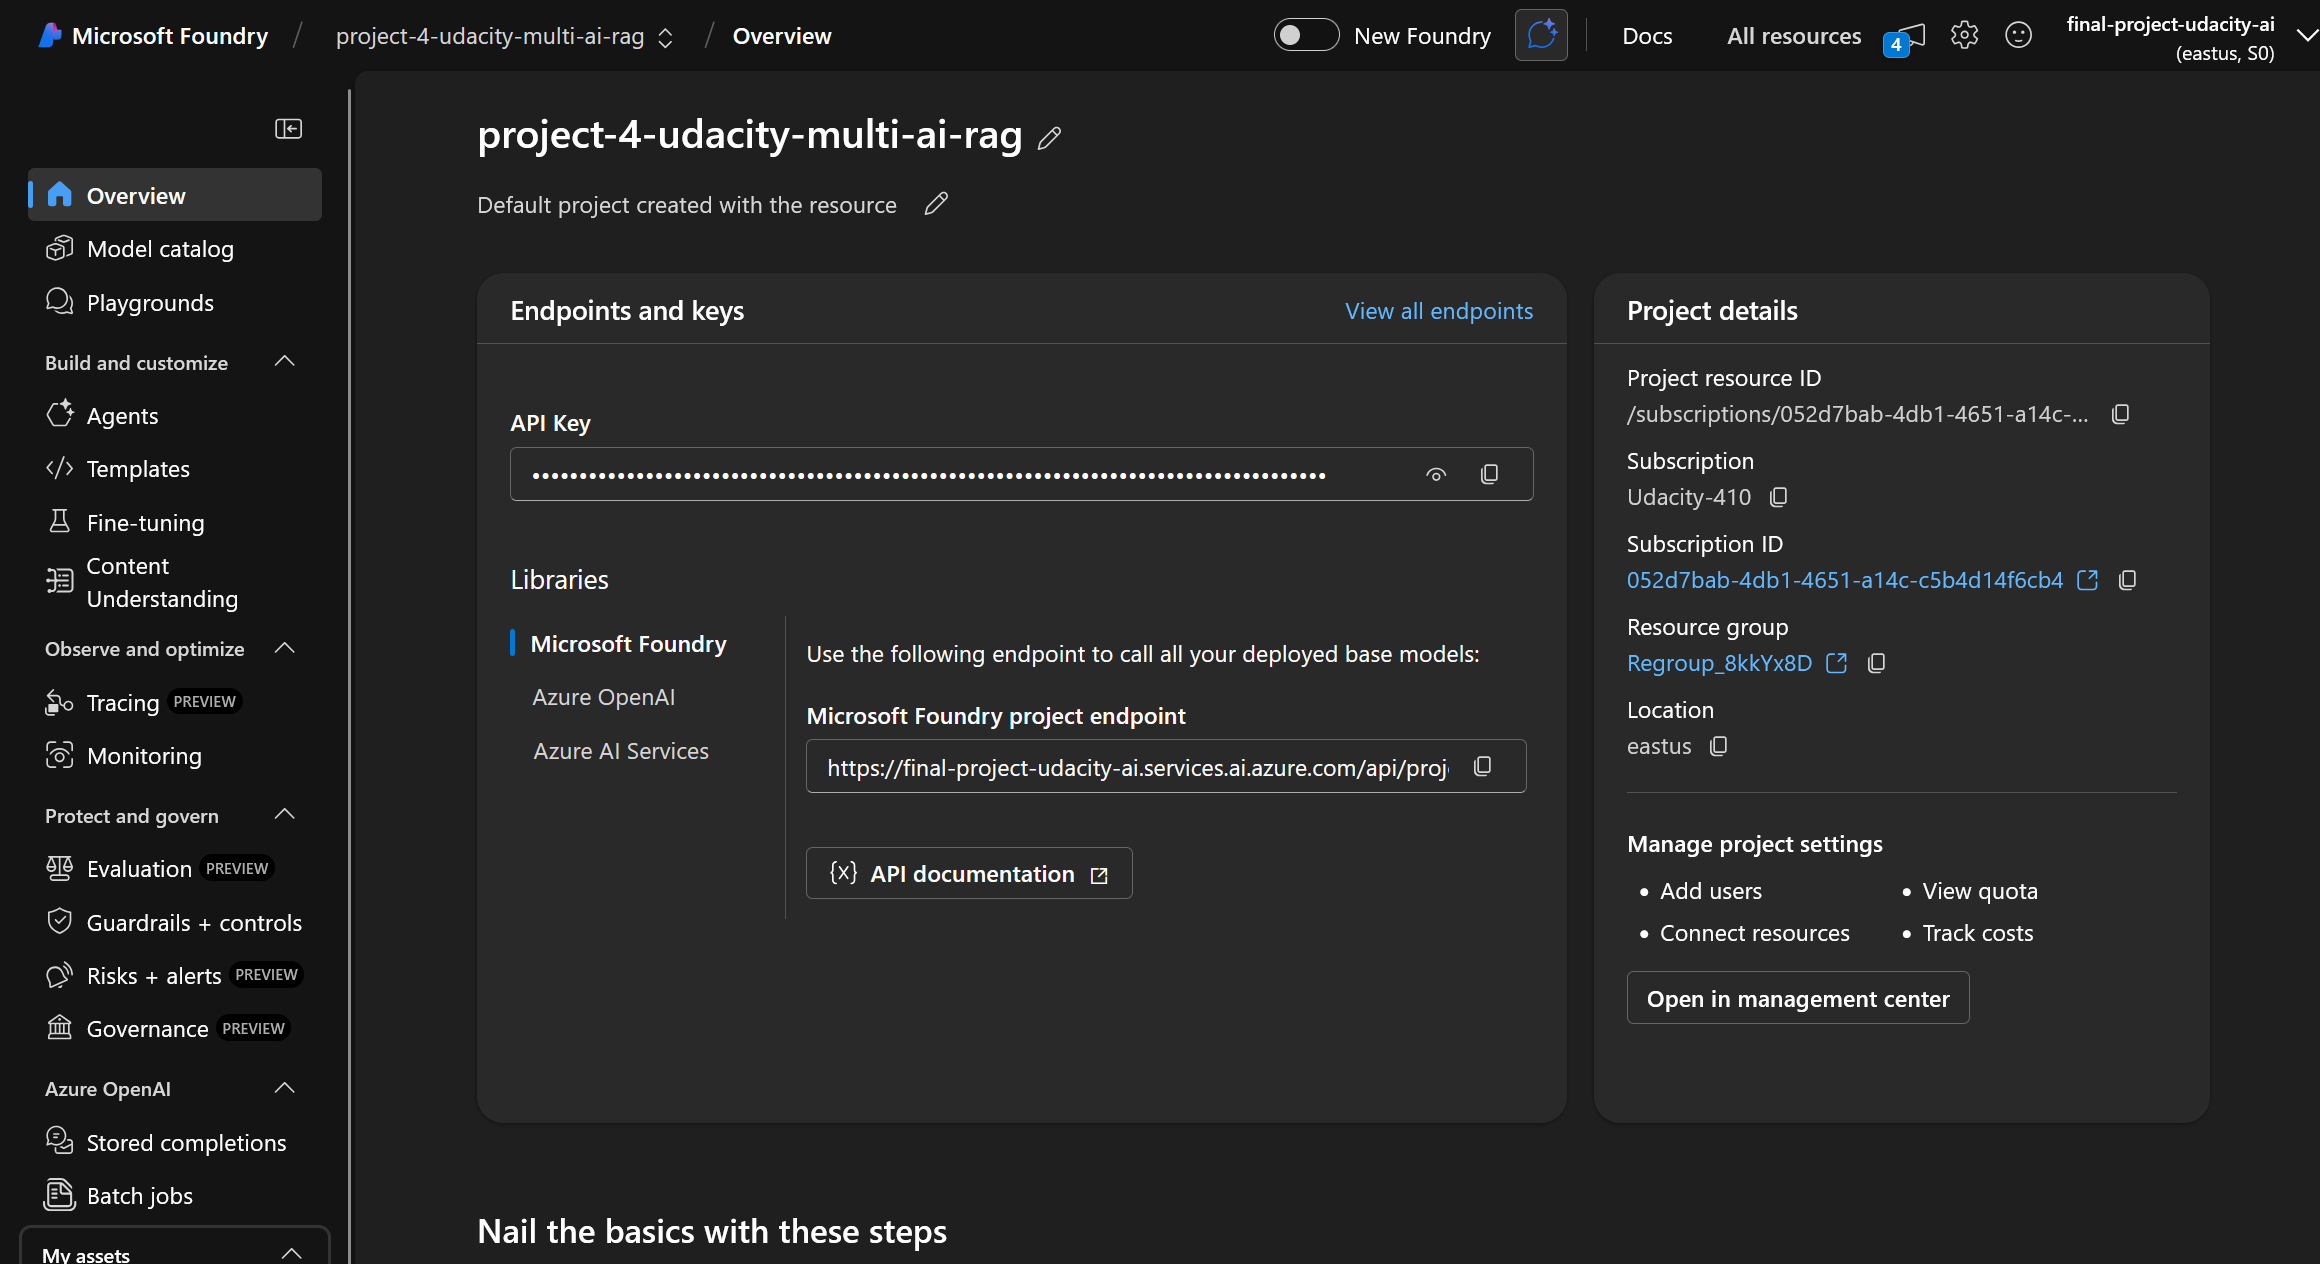
\includegraphics[width=\textwidth]{azure_openai_keys.png}
\caption{Azure OpenAI -- Keys and Endpoint Configuration}
\end{figure}

\subsection{Deployed Models in Foundry}
\begin{figure}[H]
\centering
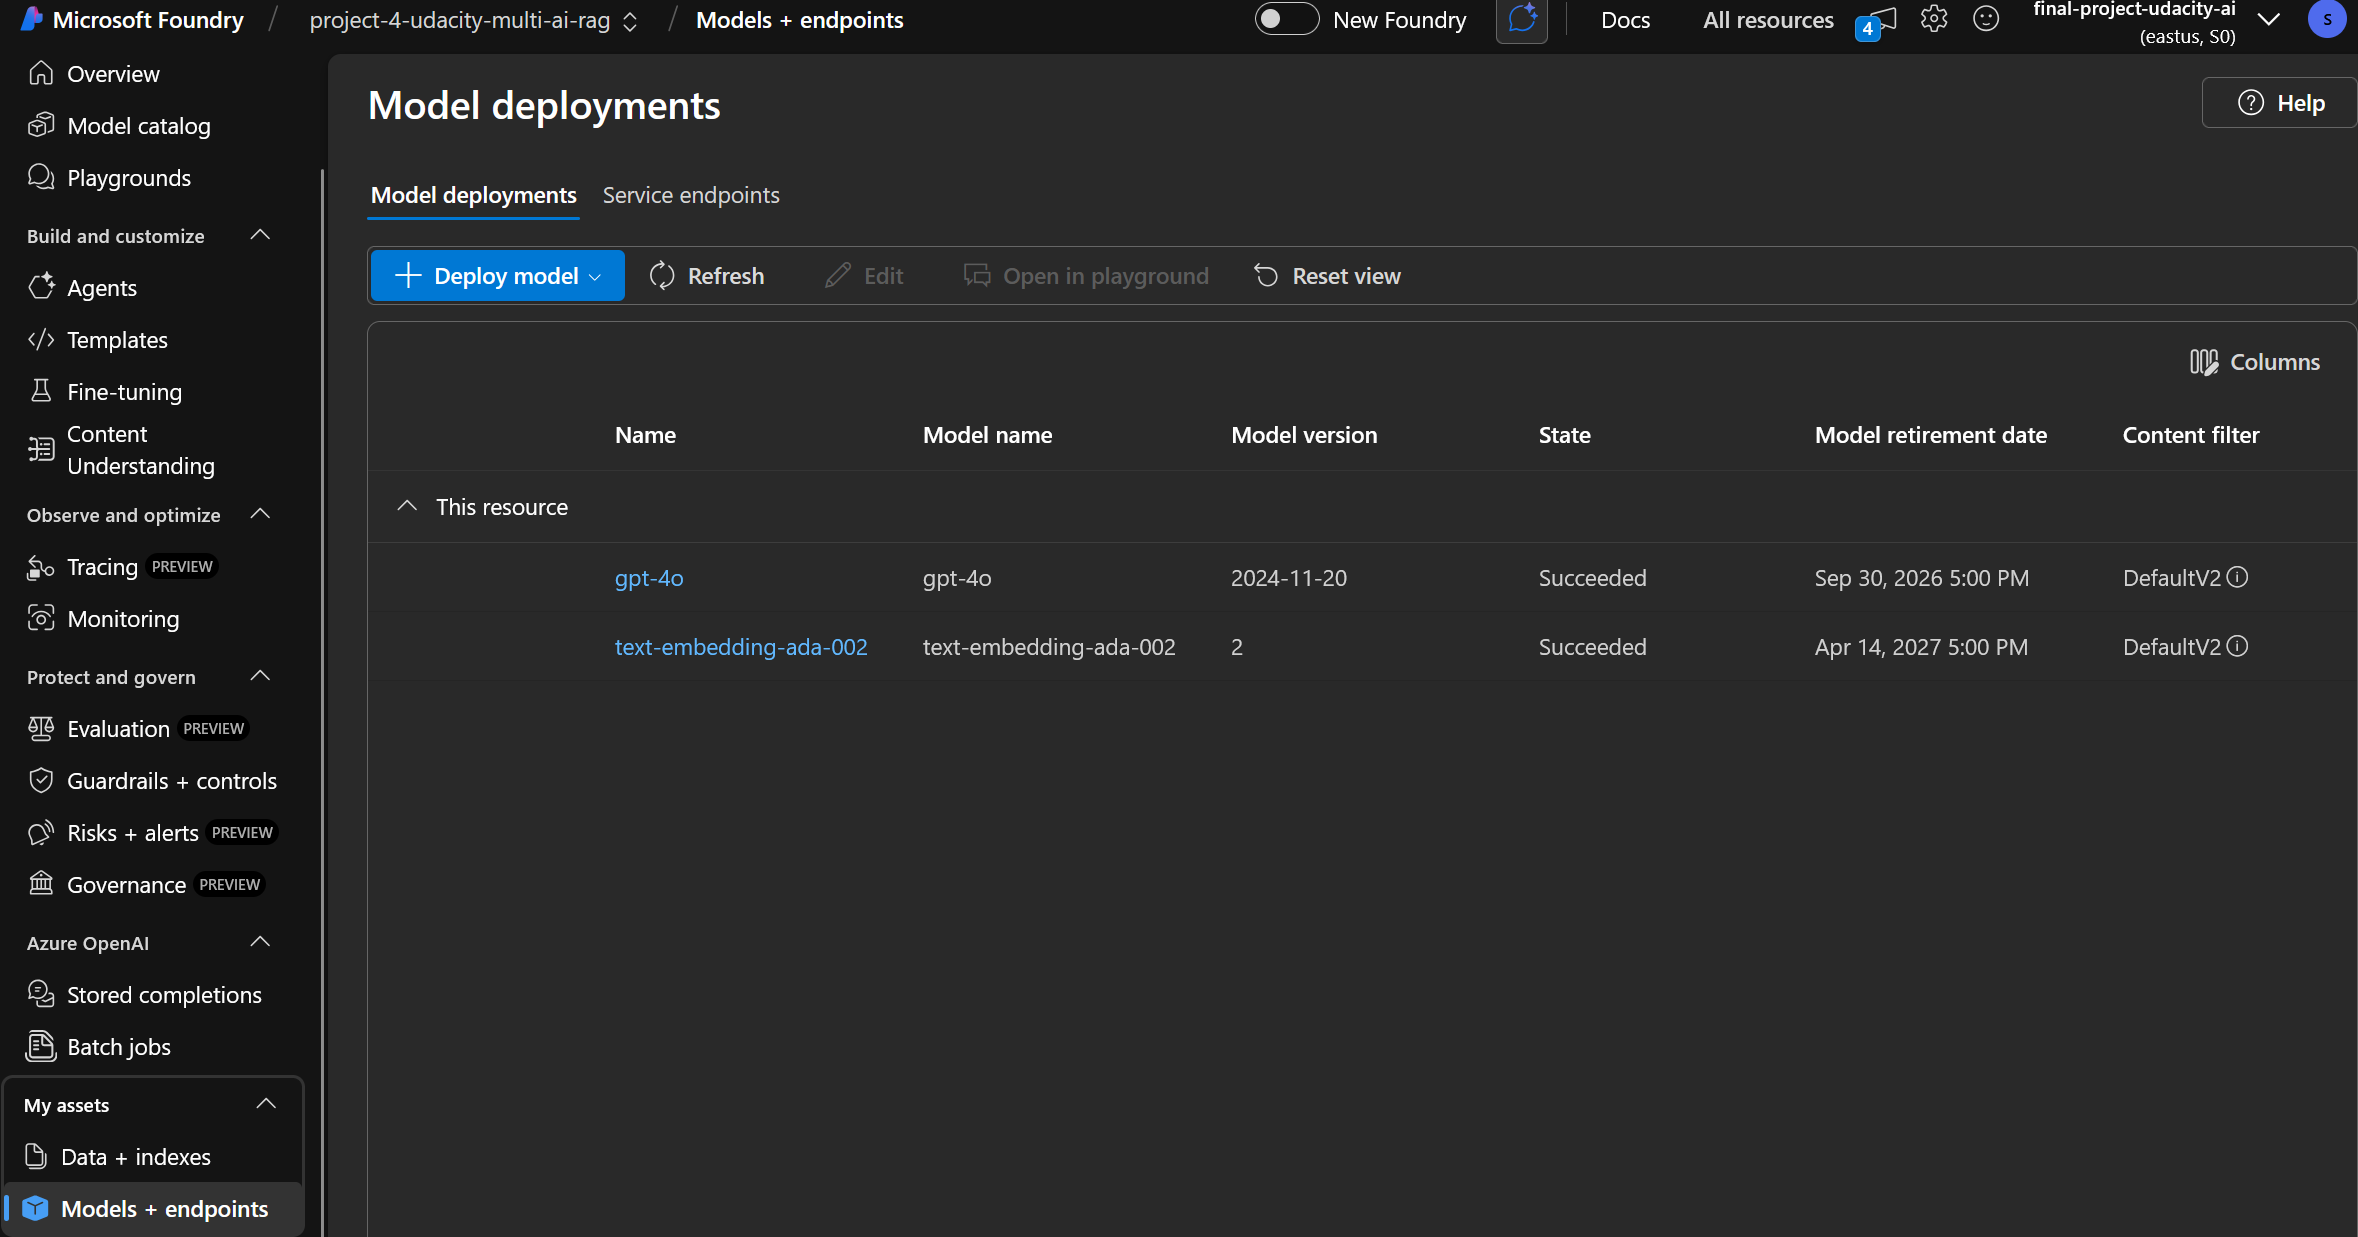
\includegraphics[width=\textwidth]{Deployed_Models_Foundry.png}
\caption{Azure AI Foundry -- Deployed Models Overview}
\end{figure}

\subsection{Azure SQL Server -- Overview}
\begin{figure}[H]
\centering
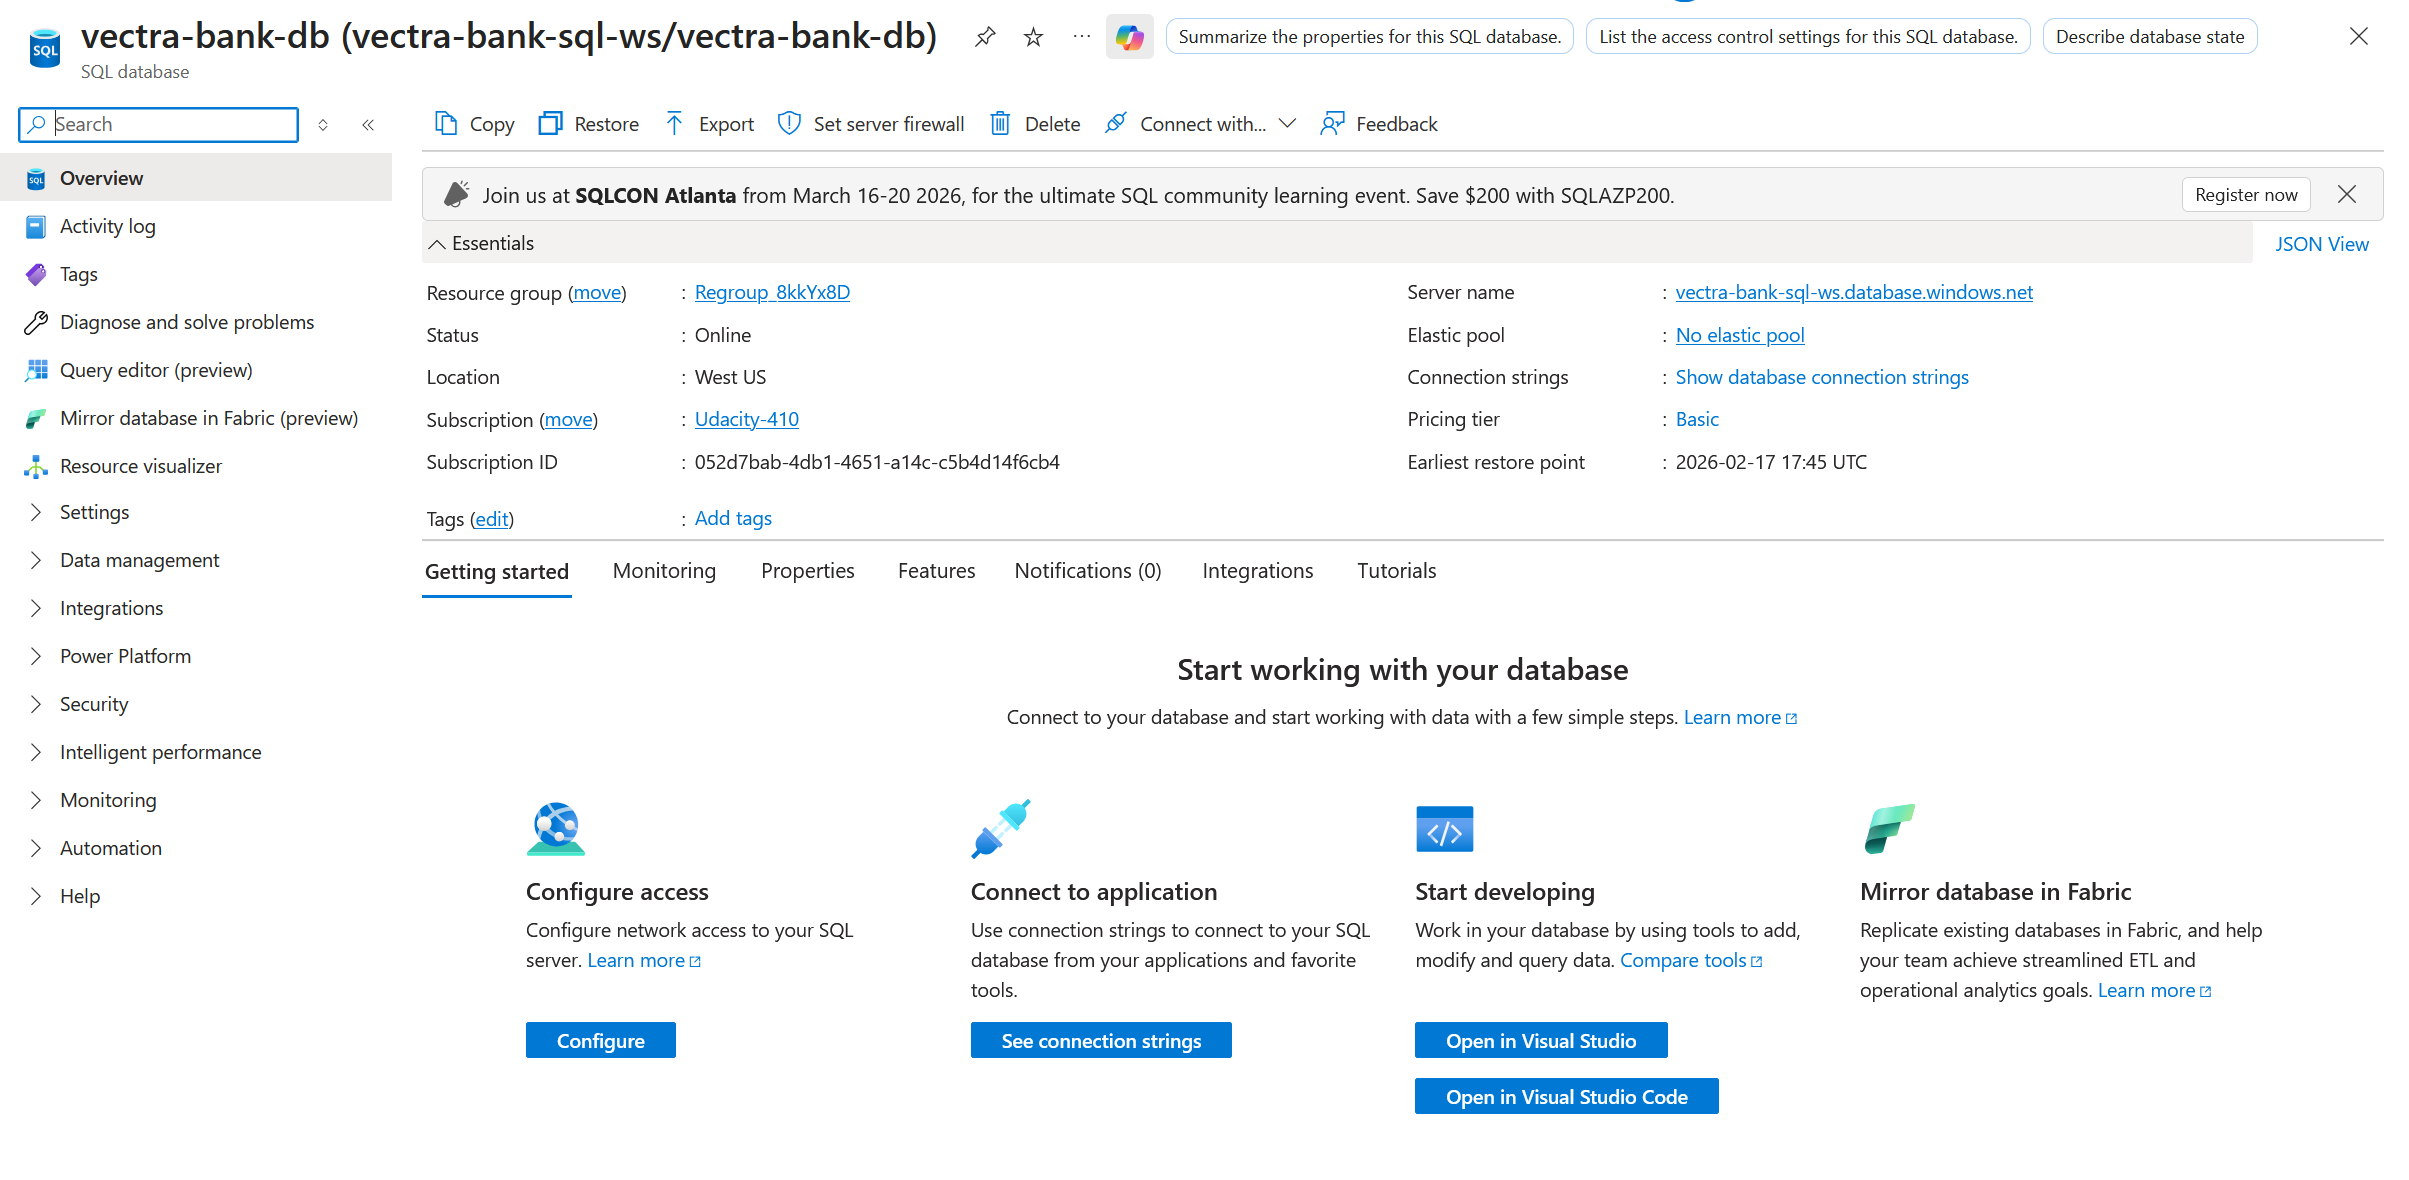
\includegraphics[width=\textwidth]{azure_sql_overview.png}
\caption{Azure SQL Server -- Resource Overview}
\end{figure}

\subsection{Azure SQL Server -- Workspace}
\begin{figure}[H]
\centering
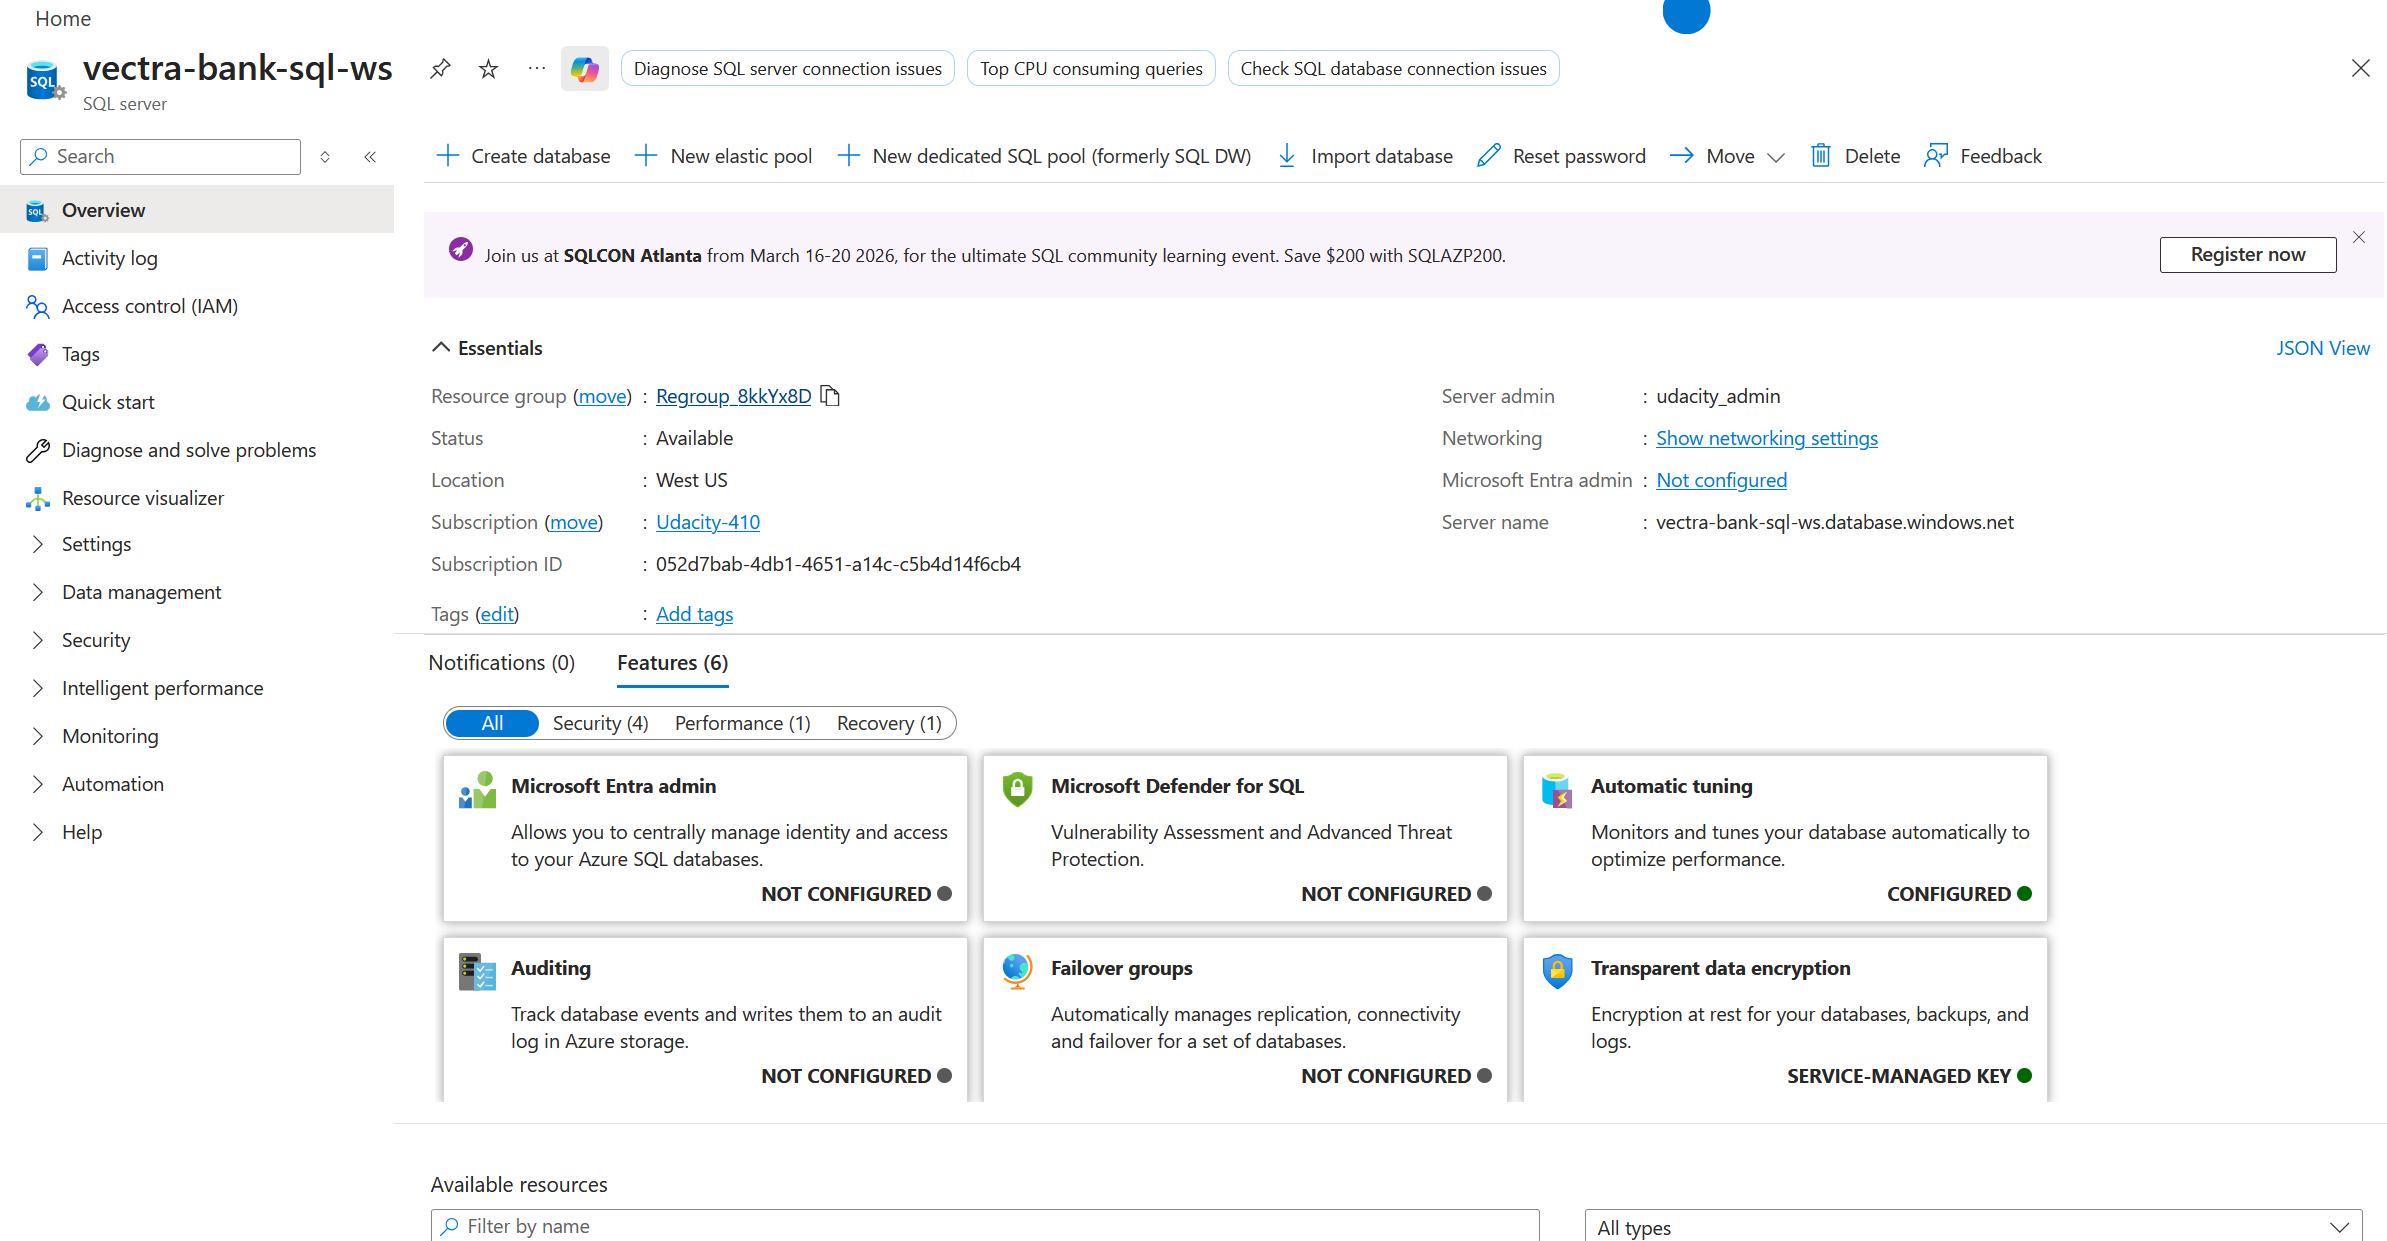
\includegraphics[width=\textwidth]{vectra_bank_sql_ws.png}
\caption{Azure SQL Server -- Vectra Bank Workspace}
\end{figure}

\subsection{Azure SQL -- Firewall Rules}
\begin{figure}[H]
\centering
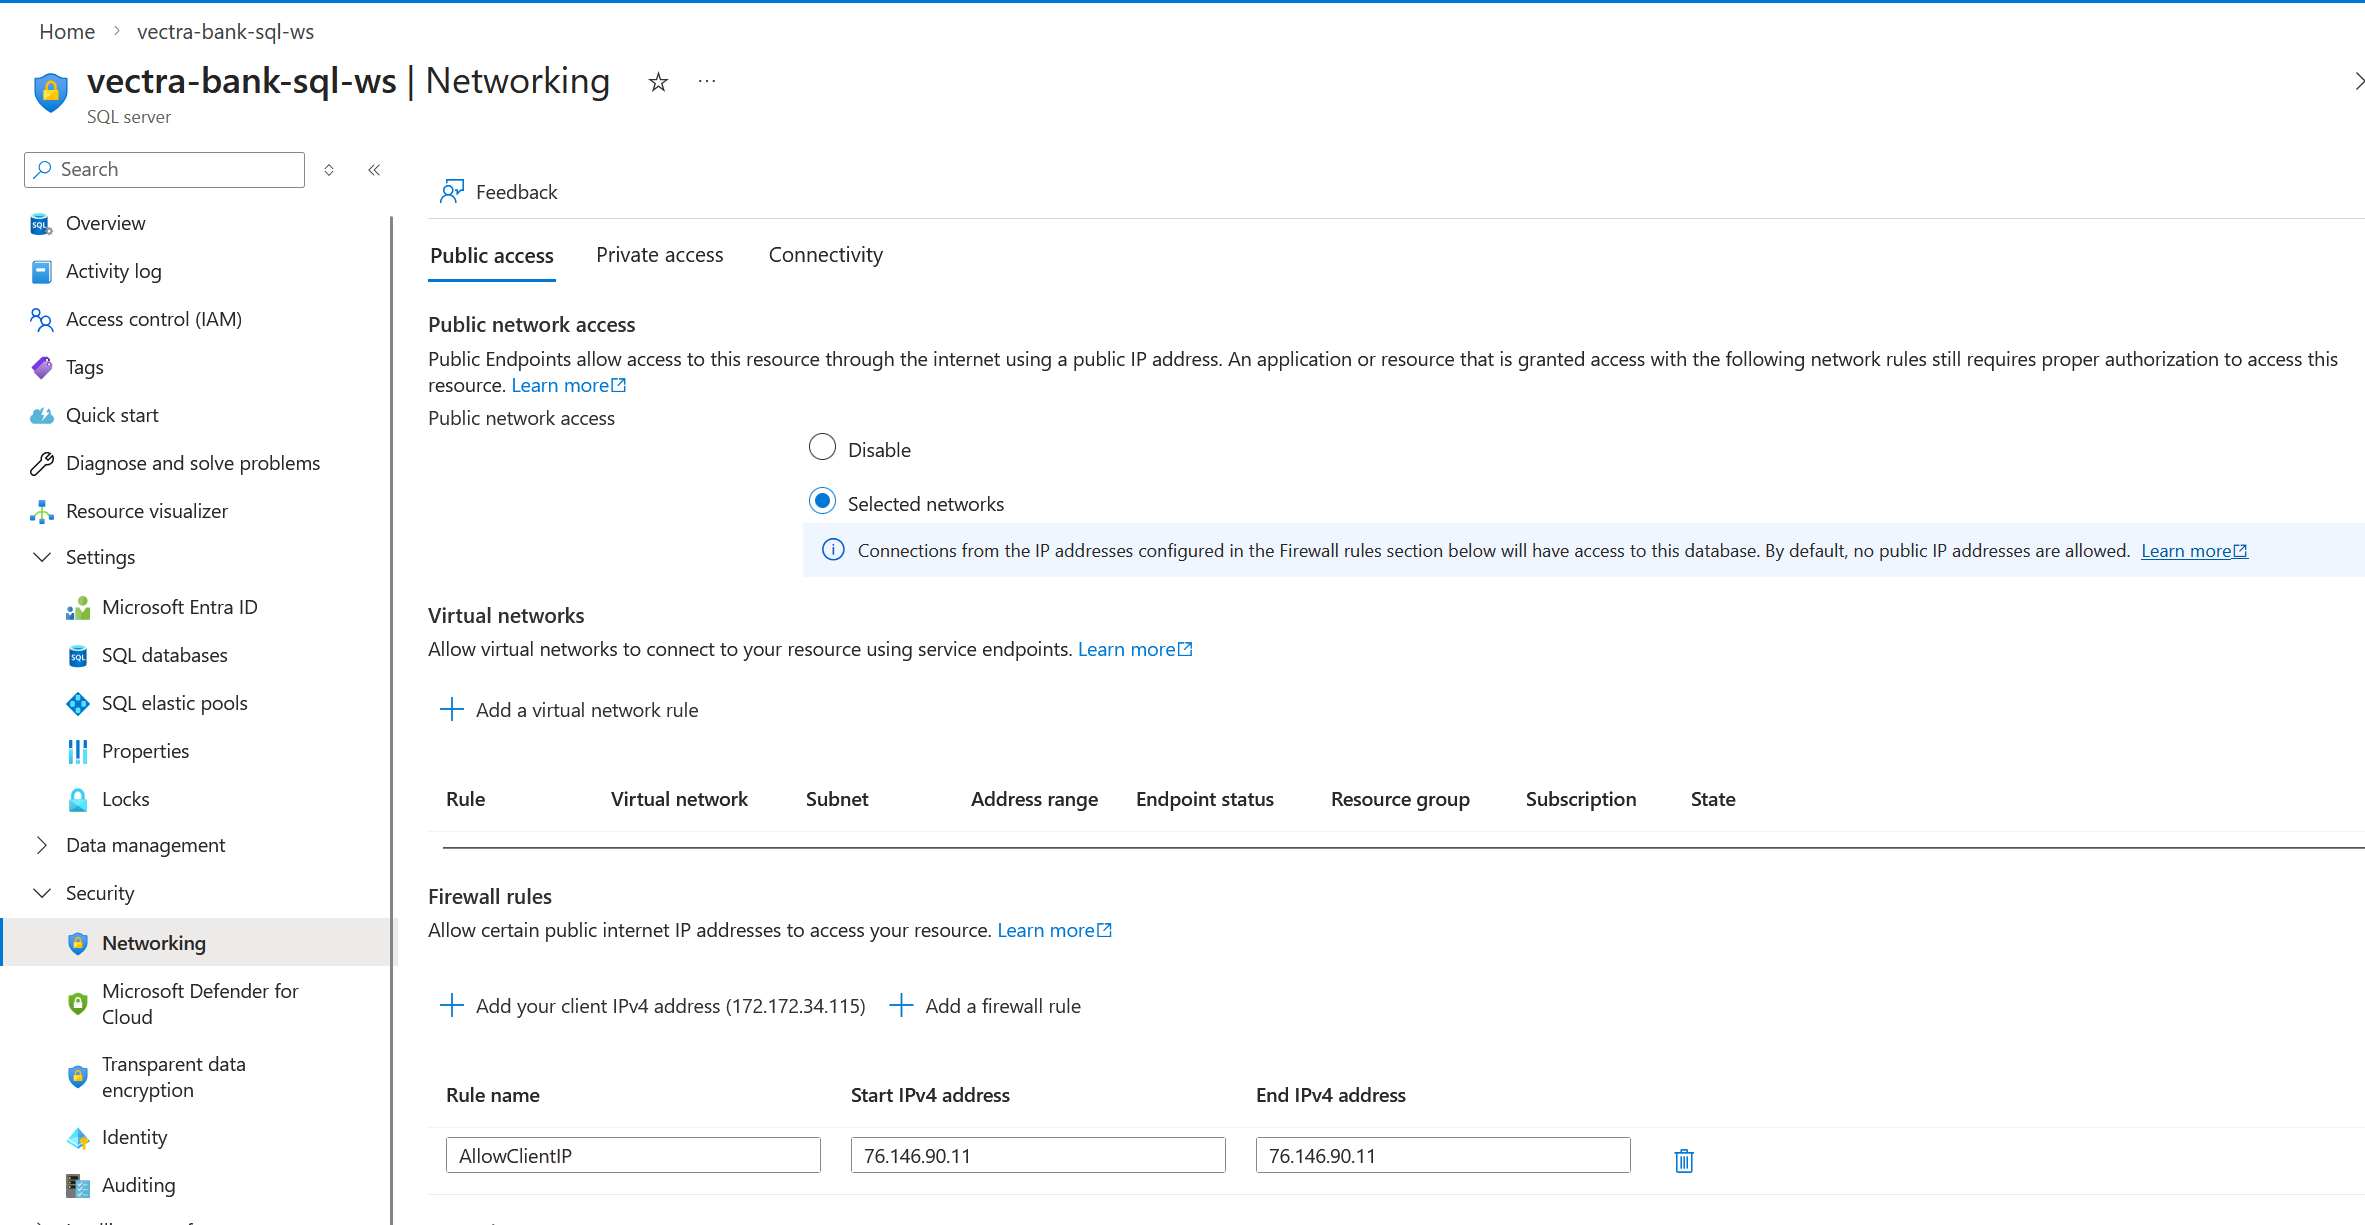
\includegraphics[width=\textwidth]{azure_sql_firewall.png}
\caption{Azure SQL -- Firewall and Networking Rules}
\end{figure}

\subsection{Azure SQL -- Query Editor}
\begin{figure}[H]
\centering
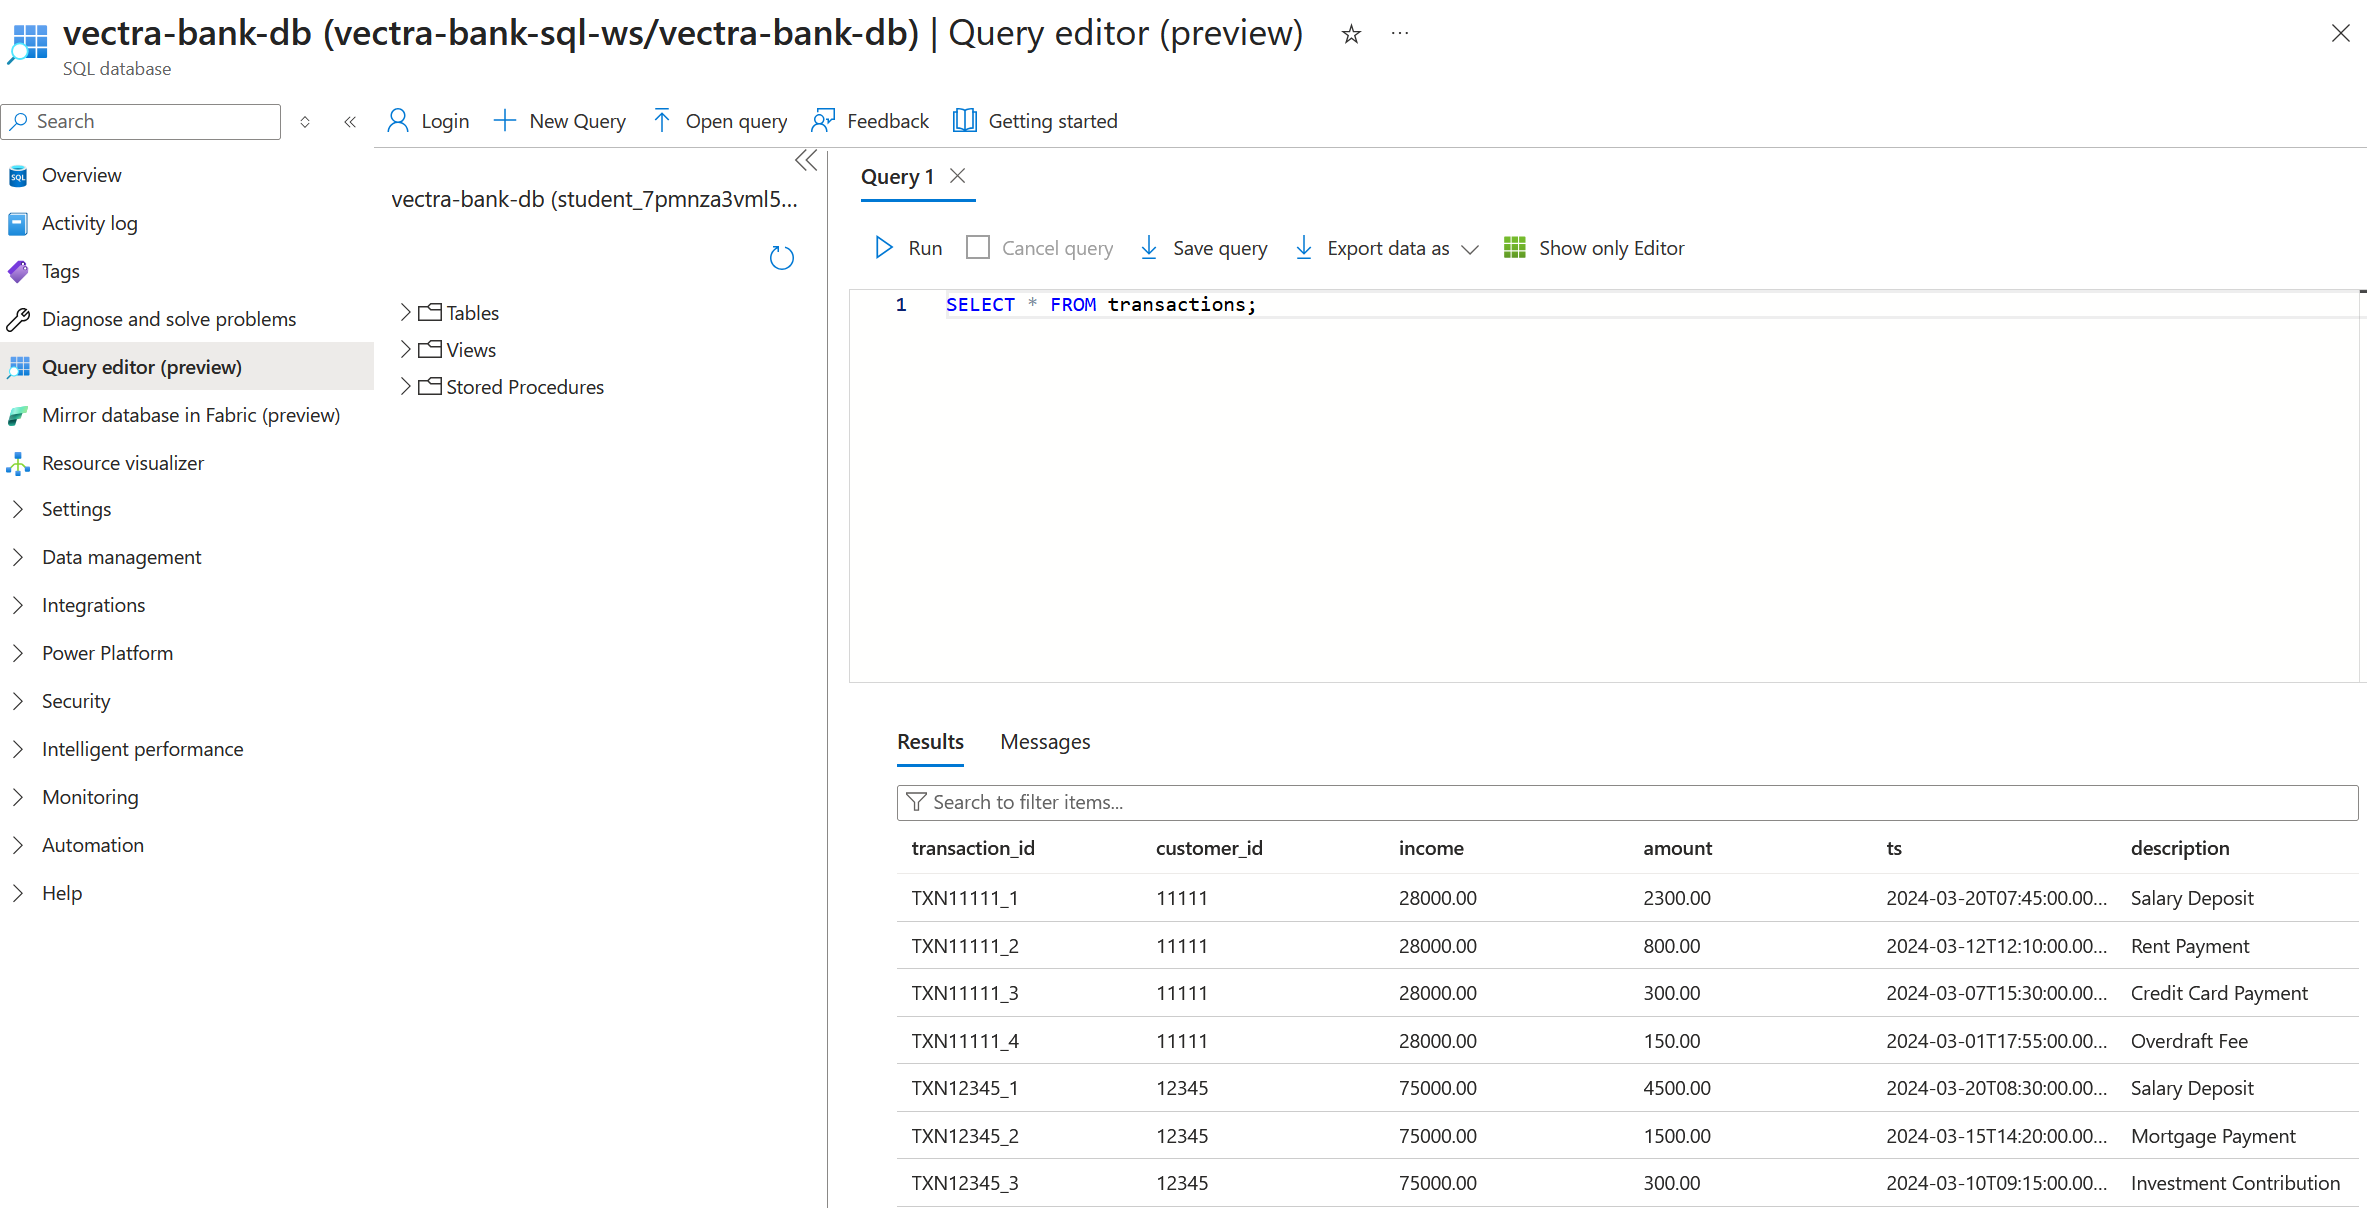
\includegraphics[width=\textwidth]{azure_sql_query_editor.png}
\caption{Azure SQL -- Query Editor showing customer transactions}
\end{figure}

\subsection{Azure SQL -- Table Schema}
\begin{figure}[H]
\centering
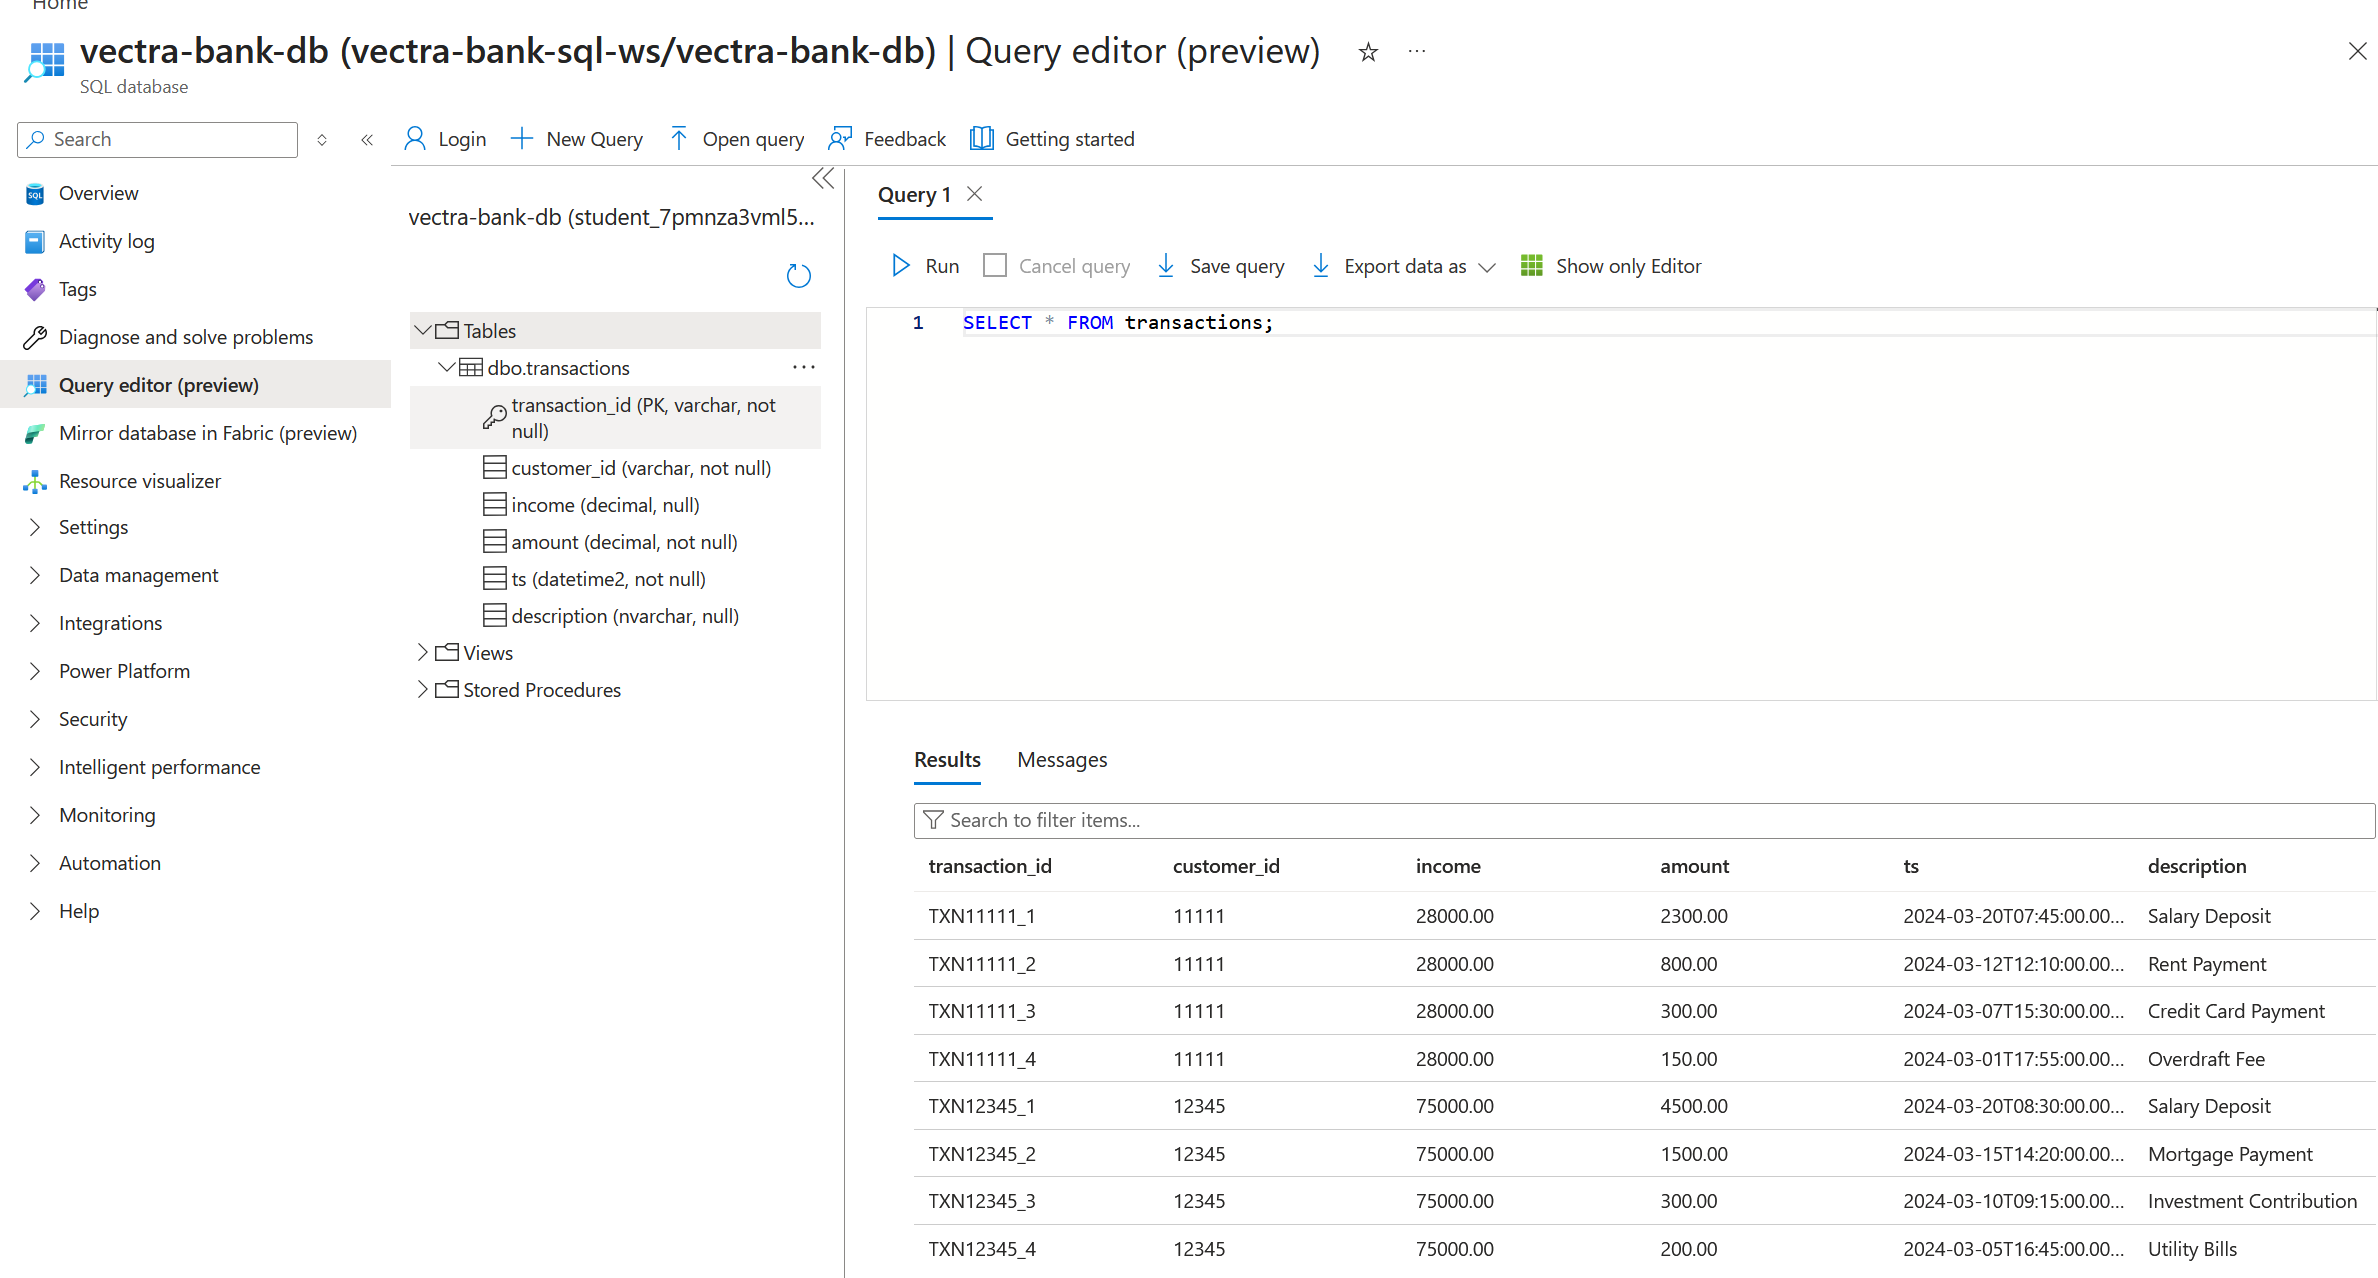
\includegraphics[width=\textwidth]{azure_sql_table_schema.png}
\caption{Azure SQL -- Table Schema for customer\_transactions}
\end{figure}

% ============================================================================
% SCREENSHOTS -- SYSTEM OUTPUT
% ============================================================================
\newpage
\section{Appendix B: System Output Screenshots}

\subsection{Test Results (23/23 Pass)}
\begin{figure}[H]
\centering
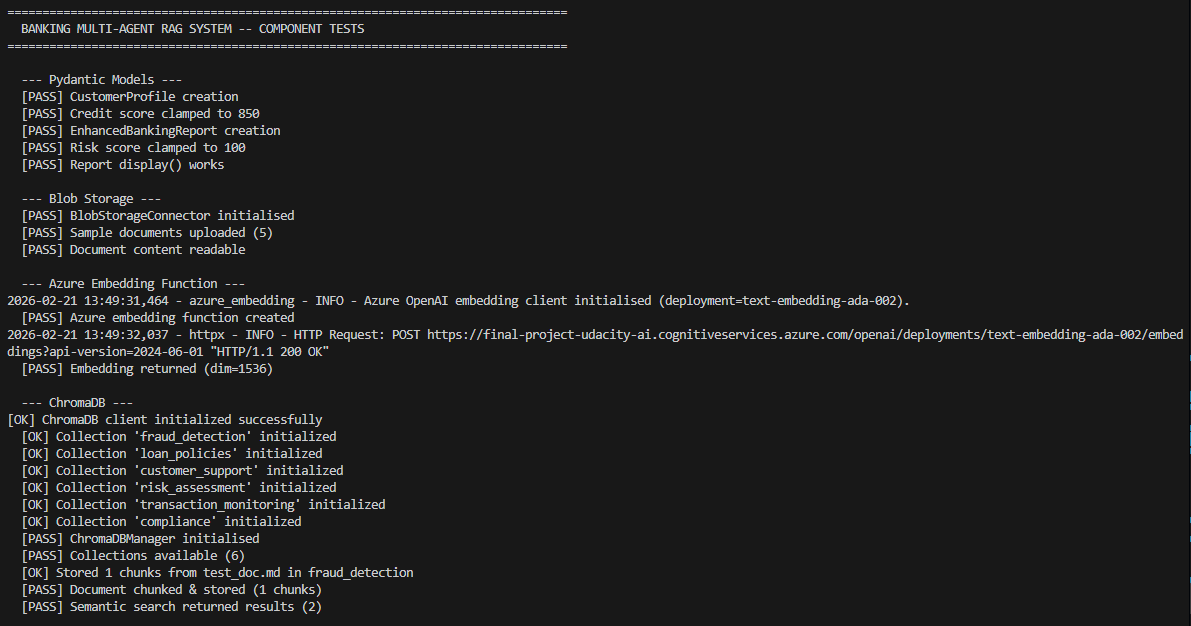
\includegraphics[width=\textwidth]{test_results_1.png}
\caption{Test Results -- Part 1: Model, Blob, Embedding, ChromaDB, RAG tests}
\end{figure}

\begin{figure}[H]
\centering
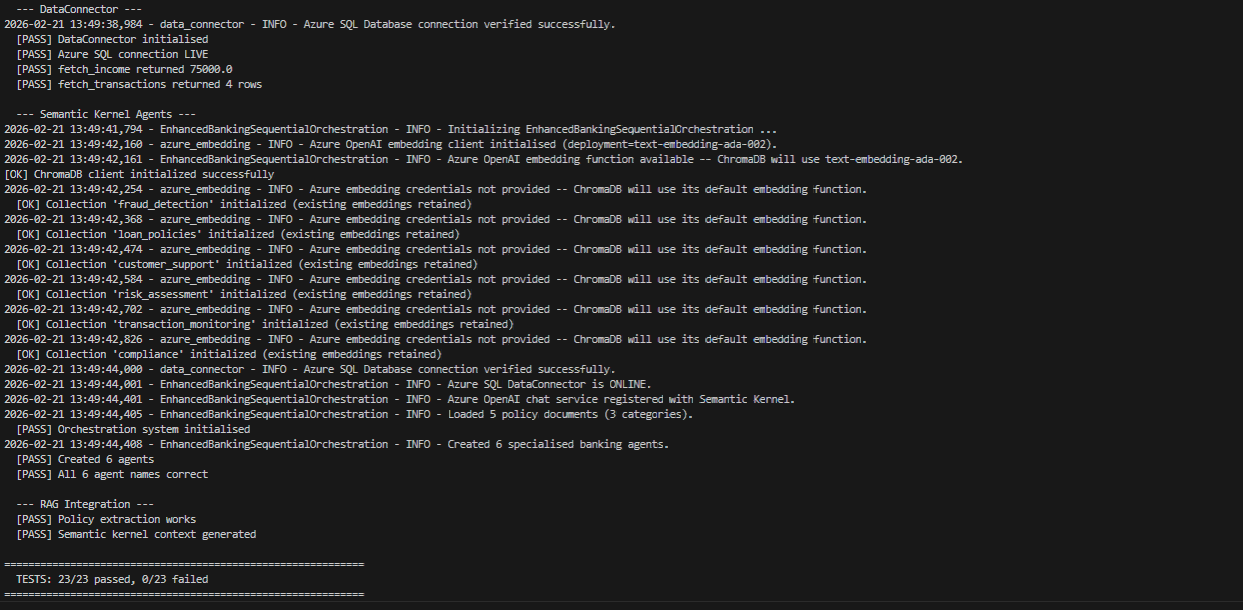
\includegraphics[width=\textwidth]{test_results_2.png}
\caption{Test Results -- Part 2: SQL, Orchestration tests and summary (23/23)}
\end{figure}

\subsection{Demo Output (Single Scenario)}
\begin{figure}[H]
\centering
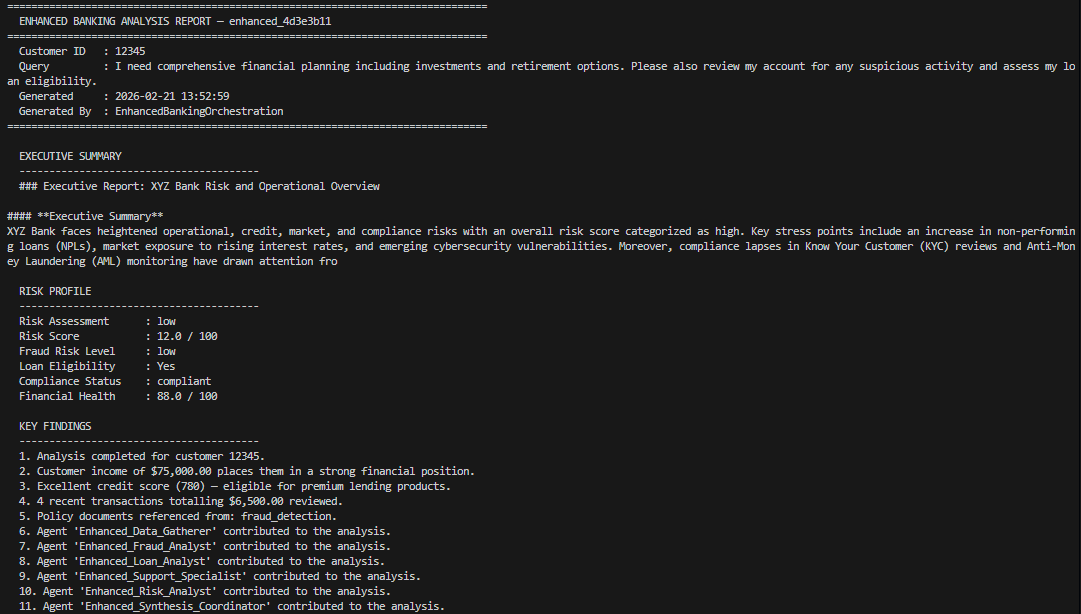
\includegraphics[width=\textwidth]{demo_output_1.png}
\caption{Demo Output -- Part 1: Agent activations and processing}
\end{figure}

\begin{figure}[H]
\centering
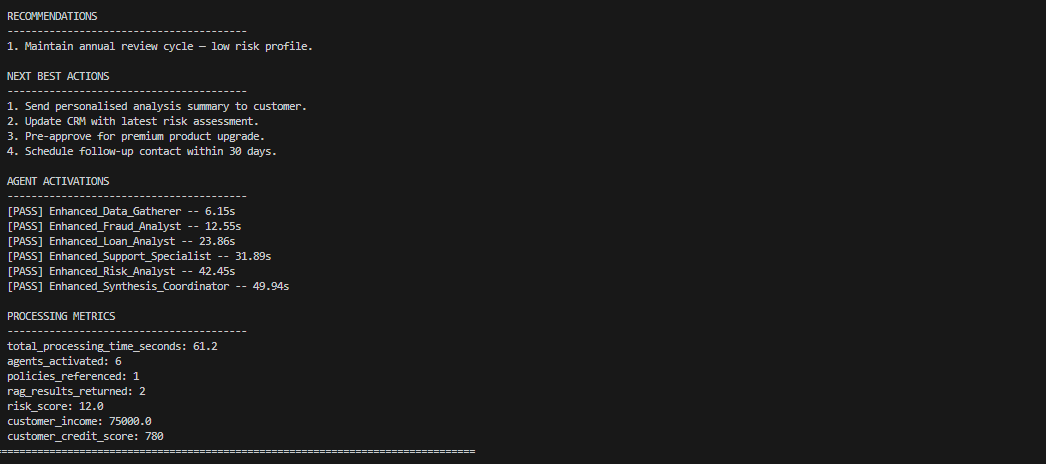
\includegraphics[width=\textwidth]{demo_output_2.png}
\caption{Demo Output -- Part 2: Final report with risk assessment}
\end{figure}

\subsection{Evaluation Output (5/5 Scenarios Pass)}
\begin{figure}[H]
\centering
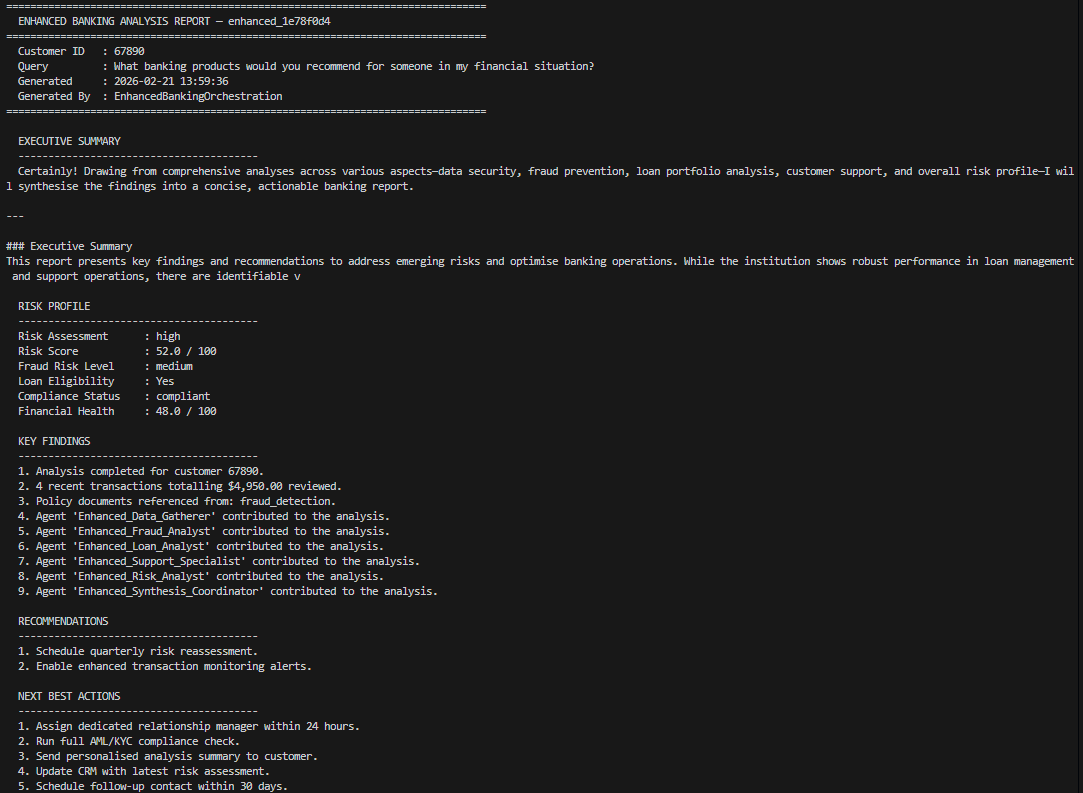
\includegraphics[width=\textwidth]{report_sample_1.png}
\caption{Evaluation Output -- Part 1: Scenarios processing}
\end{figure}

\begin{figure}[H]
\centering
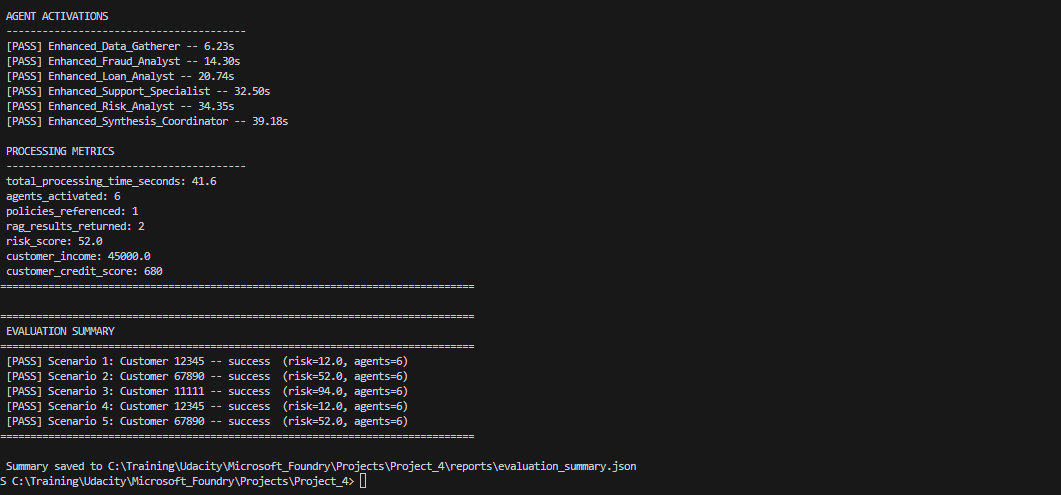
\includegraphics[width=\textwidth]{report_sample_2.png}
\caption{Evaluation Output -- Part 2: All 5 scenarios PASS summary}
\end{figure}

\subsection{Report Sample (JSON)}
\begin{figure}[H]
\centering
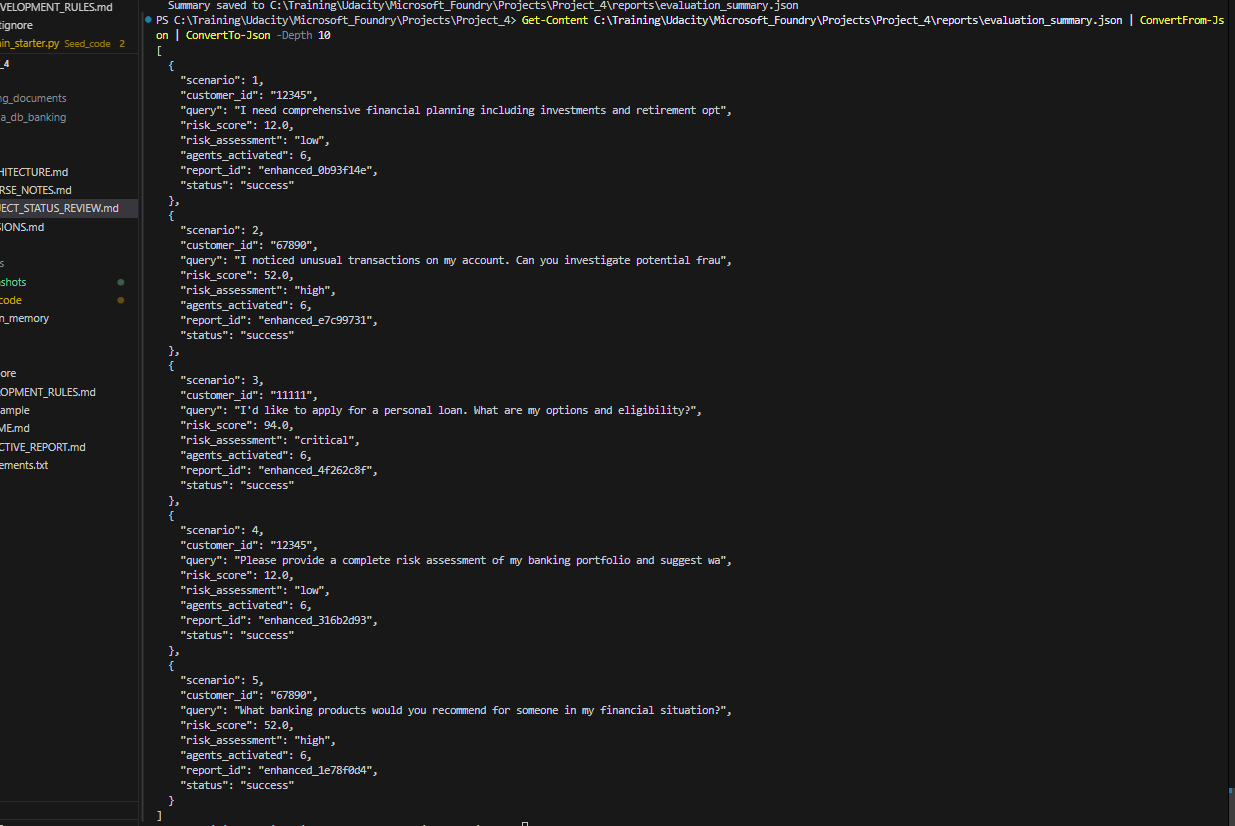
\includegraphics[width=\textwidth]{report_summary_scenarios.png}
\caption{Evaluation Summary JSON -- All 5 scenarios with risk scores}
\end{figure}

\end{document}
